%**********************************************************************
% Base layout + including standard packages
%**********************************************************************
\documentclass[a4paper,12pt]{report}
\usepackage[german,ngerman,english]{babel}
\usepackage[utf8]{inputenc}	% allows direct input of special chars
\usepackage{setspace}		% permits to set space between lines

% ensure proper appearance of all fonts in pdf:
\usepackage[T1]{fontenc}
%\usepackage{lmodern}		% lmodern after T1 fontenc (_may_ be required)
%\usepackage{times} -- obsolete; use:
\usepackage{mathptmx}		% Times as default text font, maths support
\usepackage{courier}		% provides bold font (required for syntax highlighting in listings)

\usepackage{multirow}		% enables table cells to span multiple rows

\usepackage{parskip}		% paragraphs: no indentation at beginning, but spacing between

\usepackage[pdftex]{graphicx}
\DeclareGraphicsExtensions{.pdf,.jpg,.png}


%**********************************************************************
% Including non-standard packages
%**********************************************************************

\usepackage{acronym}

\usepackage[usenames,dvipsnames,table]{xcolor}	% http://en.wikibooks.org/wiki/LaTeX/Colors
\definecolor{gray20}{gray}{0.8}
\definecolor{gray5}{gray}{0.95}
\definecolor{olivegreen30}{RGB}{155,187,89}	% from table template in MS Word

\usepackage{alltt}

\usepackage{listings}
\lstset{numbers=left, basicstyle=\tiny\ttfamily,	% numbers=none if required
	showstringspaces=false, language=C++, frame=lines
	captionpos=b, breaklines=false, numbersep=5pt}	% captionpos=b: caption at bottom

% Geometry as defined by FH guidelines:
\usepackage[top=3cm, bottom=3cm, left=3.5cm, right=3cm]{geometry}

%\usepackage{paralist} 		% inline lists
%\usepackage{mdwlist}
\usepackage{enumitem}

\usepackage{float}
\floatstyle{plain}
\restylefloat{figure}
\usepackage{subfig}

\usepackage{textcomp}		% symbols such as \texttimes and \texteuro
%\usepackage{amssymb}		% math. symbols from the American Mathematical Society

%\usepackage[Lenny]{fncychap}	% chapter heading styles


% Biblatex
% ---------------------------------------------------------------------
\usepackage[autostyle]{csquotes}		% context sensitive quotation; recommended for usage with Biblatex
% Note: date, origdate, eventdate, and urldate require yyyy-mm-dd format
% dd or mm-dd may be omitted
\usepackage[
    backend=bibtex,
    urldate=long,		% default: short, e.g. 08/15/2010
    style=authoryear,	% Harvard citation style
%   sorting=nty		this is default: sort by name, title, year
    sortlocale=de_DE	set according to your needs
    natbib=true,		% if you want to use natbib compatible citation commands; do _not_ use package natbib!
    maxbibnames=1000,		% show all authors in the bibliography
%    citestyle=alphabetic,
]{biblatex}
% Strict Harvard style: URL date default is "(Visited on ...)"; so:
% These two BibTeX entries
%	url = {http://...},
%	urldate = {2015-03} -- or 2015, or 2015-03-31
% shall be printed as
%	Available from: <http://...> [March 2015]
\DeclareFieldFormat{urldate}{\mkbibbrackets{#1}}
\DeclareFieldFormat{url}{Available\space from\addcolon\space <\url{#1}>}
\addbibresource{bac1.bib}
% ---------------------------------------------------------------------

\usepackage[			% hyperref should be last package loaded
    pdftex,			% driver
    pdftitle={Entwicklung eines beispielhaften Software-Entwicklungsprozesses für regulierte Anwendungen},
    pdfsubject={Bachelorarbeit},
    pdfauthor={Mario Löfler},
    breaklinks,			% permits line breaks for long links
    bookmarks,			% create Adobe bookmarks
    bookmarksnumbered,		% ... and include section numbers
    linktocpage,		% "make page number, not text, be link on TOC ..."
    colorlinks,			% yes ...
    linkcolor=black,		% normal internal links;
    anchorcolor=black,		% don't make scientific papers too much colourful => "black"
    citecolor=black,
    urlcolor=black,		% quite common
    pdfstartview={Fit},		% "Fit" fits the page to the window
    pdfpagemode=UseOutlines,	% open bookmarks in Acrobat
    plainpages=false,		% avoids duplicate page number problem
    pdfpagelabels,
  ]{hyperref}

%**********************************************************************
% Layout adjustments
%**********************************************************************

% page layout (header/footer and page numbers)
%\pagestyle{empty}
\pagestyle{headings}
%\pagestyle{fancy}

% settings for structure
\setcounter{secnumdepth}{3}
%\setcounter{tocdepth}{2}
\setcounter{tocdepth}{1}

%**********************************************************************
% LaTeX macros and commands
%**********************************************************************

% new command to start a chapter (no page number)
\newcommand{\chapterstart}{\thispagestyle{empty}}

% new command to close a chapter (flush, i.e. print remaining figures and tables)
\newcommand{\chapterend}{\newpage{\pagestyle{empty}\cleardoublepage}}

% new environment for smaller paragraphs
\newenvironment{spar}
{\begingroup \leftskip 0.7cm \rightskip\leftskip}
{\par \endgroup}
% ^^^ must be set here (or use empty line)


%**********************************************************************
% Special hyphenation rules
%**********************************************************************

\hyphenation{JOANNEUM}		% extend to your needs

\newcommand{\code}[1]{\mbox{\texttt{#1}}}

%**********************************************************************
% Structure of thesis: inclusion of chapters
%**********************************************************************

\begin{document}

  %**********************************************************************
% right side, if two-sided
\chapterend
\selectlanguage{german}
\begin{titlepage}

\begin{center}
% scale image according to the actual logo you use
% official JPG ist way too large, so [height=2.5cm] is required
% official EPS, converted to PDF:

\includegraphics[height=1cm]{images/logo_FHJ_100mm_cmyk}
\hfill

% the actual title
\mbox{}\vfill

  \large

  {\huge\bf Implementierung eines \\persistenten und skalierenden\\Job-Schedulers}

  \vspace{2.0cm}

  {\bf Bachelorarbeit 2}\\
{\bf zur Erlangung des akademischen Grades\\ Bachelor of Science in Engineering (BSc)}\\
eingereicht am\\
Fachhochschul-Studiengang {\bf Software Design} 


  \vspace{0.5cm}

 FH JOANNEUM  (University of Applied Sciences), Kapfenberg

  \vspace{1.5cm}

  \mbox{}

  {\bf Betreuer: FH-Prof. Dipl.-Ing. Dr. Egon Teiniker

  eingereicht von: Mario Löfler\\
  Personenkennzahl: 1310418017}

  \vspace{1.5cm}

   Juni 2017

\end{center}
\vfill\mbox{}


\end{titlepage}



%**********************************************************************

% right side/flush
\chapterend






\chapterend


  \pagenumbering{roman}		% roman page numbers for title pages

\begin{titlepage}
	\selectlanguage{german}
\begin{abstract}
	
Die wiederkehrende Erledigung von Aufgaben ist in der EDV ein häufig anzutreffendes Problem. Dabei müssen die Aufgaben in etwa zu einem bestimmten Zeitpunkt in der Zukunft erledigt werden oder wiederkehrend in vorgegebenen Zeitabständen ausgeführt werden - ohne Interaktion eines Benutzers.\\
Im Internet der Dinge werden solche Systeme auch oft eingesetzt um Daten von Geräten zu holen die diese nicht aktiv zur Verfügung stellen können. Im Internet der Dinge kann diese Anzahl dabei rasch hoch werden, das System muss mit der wachsenden Anzahl an Geräten in der Leistungsfähigkeit mitwachsen und die erwarteten Tätigkeiten ausführen.\\
In dieser Arbeit wird ein solches System das sowohl funktionell als auch in der Leistung skaliert entwickelt und prototypisch eingesetzt. Einige der wichtigen Themen werden auch in der Theorie erklärt und die Umsetzung im Code erläutert. Schwerpunkt dieser Erläuterungen sind insbesondere die Problemstellungen bei der Persistenz der durchzuführenden Aufgaben und der Sicherstellung der Leistung.\\
Die Umsetzung wird zur Lösung einer tatsächlichen Aufgabenstellung eingesetzt. Der Theorieteil basiert auf einer Literaturrecherche.\\
Zielpublikum der Arbeit sind Entwickler die an Serversystemen arbeiten die wiederkehrende Aufgeben zu erledigen haben oder ähnliche Problemstellungen im Bereich der Skalierung zu erfüllen haben.
\end{abstract}


\selectlanguage{english}
\begin{abstract}

Recurring tasks are a common challenge in software systems. Tasks either need to be scheduled to be executed at a future point in time or need to be executed in set intervals without further user interaction.\\
The Internet of things often uses such systems to fetch data from devices that can not actively push the data. The number of devices within the Internet of things is often large and heterogeneous, so the tasks that need to be run are diverse. The system therefore needs to be able to scale in performance and functionality.\\
As a part of this thesis such a system is developed put to use in a real environment. Exemplary problems like persistence and concurrency are elaborated in this thesis. The theoretical part is backed by literature research.
The target audience of this theses are developers that either face the challenge of recurring tasks or are generally interested in the scaling problems.

\end{abstract}
\selectlanguage{german}
\end{titlepage}
	\chapterend
\begin{titlepage}
	\selectlanguage{german}
\begin{titlepage}

%-t-\parindent0pt
%-t-\parskip1.5ex plus.5ex minus.5ex

\begin{center}\large\bf
Ehrenwörtliche Erklärung
\end{center}

Ich erkläre ehrenwörtlich, dass ich die vorliegende Bachelorarbeit
selbstständig angefertigt und die mit ihr verbundenen
Tätigkeiten selbst erbracht habe. Ich erkläre weiters, dass ich keine anderen
als die angegebenen Hilfsmittel benutzt habe. Alle aus gedruckten, ungedruckten
oder dem Internet im Wortlaut oder im wesentlichen Inhalt übernommenen
Formulierungen und Konzepte sind gemäß den Regeln für gutes
wissenschaftliches Arbeiten zitiert und durch Fußnoten bzw. durch andere genaue
Quellenangaben gekennzeichnet.\\\\
Die vorliegende Originalarbeit ist in dieser Form zur Erreichung eines akademischen
Grades noch keiner anderen Hochschule vorgelegt worden. Diese Arbeit
wurde in gedruckter und elektronischer Form abgegeben. Ich bestätige, dass
der Inhalt der digitalen Version vollständig mit dem der gedruckten Version
übereinstimmt.\\\\
Ich bin mir bewusst, dass eine falsche Erklärung rechtliche Folgen haben kann.

\vspace{50mm}
Graz, 21. Juni 2017 \hfill Mario Löfler

\end{titlepage}
\end{titlepage}
  \tableofcontents
  \chapterend

  \pagenumbering{arabic}	% ... for ordinary chapters
  \onehalfspacing
  \selectlanguage{german}
\chapter{Einleitung}\label{chap:Einleitung}
\chapterstart
In diesem Kapitel stelle ich das zugrundeliegende Problem vor. Aus einer allgemeinen Beschreibung werden im Zusammenspiel mit einer beispielhaften Verwendung der zu entwickelnden Software die grundlegenden Anforderungen erarbeitet. Aus diesen werden die Ziele dieser Arbeit definiert.
\section{Motivation}
Die meisten Benutzer von Computerprogrammen nutzen diese interaktiv. Sie befinden sich in einem Dialog mit der Software, wo sie aufgrund ihrer Eingabe eine bestimmte Ausgabe erwarten. Handelt es sich bei den Aufgaben die so dem Programm gestellt werden um länger laufende Aktionen, so gibt der Benutzer bloß den Anstoß, die Aufgabe selbst wird ohne weitere Interaktion erledigt und das Ergebnis angezeigt. Die meiste Zeit ist die Aufmerksamkeit des Benutzers nicht notwendig. Gibt es nun mehre Aufgabenstellungen dieser Art die wiederholt ausgeführt werden müssen, so sollten diese automatisiert werden, so dass sie ohne Eingriff des Benutzers ausgeführt werden und dieser nur mehr bei Problemen informiert wird.\\
Bei Aufgaben dieser Art handelt es sich oft um Datenimporte, bei denen aus unterschiedlichen Quellsystemen Daten geladen und in Zielsysteme importiert oder mit den Daten in Zielsystemen abgeglichen werden.\\
Die regelmäßige Ausführung von Programmen wird durch \emph{Scheduler} übernommen. Dies sind Programme die gemäß einem durch den Benutzer definierten Zeitplan Aufgaben automatisiert ausführen. Zwei der bekanntesten Vertreter sind \emph{cron} unter Linux oder der \emph{Windows Task Scheduler} für Microsoft Windows.\\
Beide Scheduler bieten eine gute Möglichkeit Programme basierend auf Zeitplänen auszuführen, beide haben jedoch die Einschränkungen dass sie
\begin{itemize}
	\item Programme nur auf einem Rechner ausführen und
	\item nur komplette Programme ausführen.
\end{itemize}
Wenn die Anzahl der Aufgaben die ausgeführt werden soll ansteigt, müssen die Aufgaben durch den Benutzer selbst auf mehrere Rechner verteilt werden. Wenn ein Rechner ausfällt oder ein neuer Rechner hinzukommt muss der Benutzer die Aufgaben ebenso neu verteilen.\\
Ebenso sind beide Scheduler darauf ausgelegt komplette Programme, also \emph{executables} auszuführen. Dadurch müssen diese für Ausführung ein neuer \emph{Prozess} angelegt werden und die dazugehörigen Daten erneut in den Speicher geladen werden. Werden nun häufig die selben Aufgaben erledigt und sind diese relativ klein, so steht der Zusatzaufwand des Ausführens meist nicht im Verhältnis zur Ausführungszeit der Aufgabe selbst.\\
Für den Fall der umzusetzen war stellten diese beiden Herausforderung ein großes Hindernis dar. Nach der Anforderungsanalyse und einer Machbarkeitsstudie wurde daher entschieden einen eigenen Scheduler umzusetzen.

\section{Beispielhafte Verwendung}
Eines der Hauptthemen in der Industrie 4.0 ist die Einbindung von Sensoren in EDV Systeme um durch deren Daten einerseits Informationen zu aktuellen (Betriebs-) Zuständen zu erhalten und andererseits durch die Sammlung der Daten mithilfe von Big-Data Algorithmen weitere Schlussfolgerungen ziehen zu können.\parencite[S. 36ff]{Manzei2015}\\
Dabei wird in der Regel stillschweigend von der neuesten Generation von Sensoren ausgegangen, die aktiv Daten in die Cloud publizieren.\footnote{Siehe zum Beispiel \parencite{ms_azureiot} "...the device sends..."} Diese Sensoren sind aktiv und lösen somit die weitere Verarbeitung der Daten aus. Es ist keine Aktivierung von Außen notwendig.\\
Viele der derzeit bestehenden Sensoren sind passiv und stellen ihre Daten nur auf Nachfrage zur Verfügung. Die Daten dieser Sensoren müssen periodisch abgefragt, und an die weiterverarbeitenden Prozesse weitergereicht werden.\\
In der beispielhaften Verwendung sollen Standbilder von bestehenden Überwachungskameras zu Dokumentationszwecken in einem Archiv abzulegen. Die Anzahl der Kameras beträgt in etwa 1.000 und wird mit der Zeit deutlich steigen, damit muss das System frei skalieren.\\ 
\section{Ziele der Arbeit}
Ziel der Arbeit ist es einen funktionstüchtigen Scheduler der auf mehreren Rechnern läuft und nicht vollständige Prozesse ausführt zu erstellen. Im Rahmen dieser Arbeit wird nur der Scheduler Kern entwickelt, die Oberflächen zum Einrichten und Verwalten der Aufgaben, sowie das Einsehen der Protokolle wird nicht umgesetzt.
\\Im Theorieteil werden die zugrundeliegenden Themen in den Bereichen Datenbanken und Concurrency\footnote{Zu Deutsch Nebenläufigkeit. Im Sinne der besseren technischen Verständlichkeit werde ich im folgenden nur den englischen Fachbegriff verwenden.} mittels Literaturrecherche erläutert.
\\ Durch diese Erläuterungen sollen die getroffenen Designentscheidungen untermauert werden und einem Entwickler die Themenkomplexe verständlich vermittelt werden.

\section{Verwendete Programmierumgebung}
Für die Umsetzung des Schedulers - und in folge auch der Implementierung der einzelnen Aufgaben - wurde das Microsoft .NET Ökosystem gewählt. Verwendet wurden
\begin{itemize}
	\item Microsoft .NET 4.6
	\item Microsoft C\# 7
	\item Microsoft Visual Studio 2017 Express Edition
	\item Microsoft Entity Framework 6 als ORM Schicht\footnote{object-relational mapping, eine Bibliothek die den Zugriff auf eine relationale Datenbank sowie die Abbildung der Daten in Klassen und Instanzen implementiert. Vgl. \parencite{ef_orm} }
	\item Microsoft SQL Server 2016 als Datenbank
\end{itemize}
Die Auswahl wurde einerseits durch meinen bisherige Erfahrung mit .NET / C\# geprägt, anderseits spielten vor allem folgende Faktoren eine entscheidende Rolle:
\begin{itemize}
	\item Lauffähigkeit unter Microsoft Windows
	\item Automatische Installierbarkeit von Sicherheitspatches für die Laufzeitumgebung
	\item Hohe Ausführungsgeschwindigkeit unter Microsoft Windows
	\item Mögliche Portierbarkeit auf andere Betriebssysteme mittels Microsoft .Net Core das zu diesem Zeitpunkt bereits in einer ersten Version zur Verfügung steht.
\end{itemize}
\section{Anforderungen}\label{chap:Anforderungen}
\subsection{Allgemein}
Wie Eingangs erwähnt, soll das System Bilder in regelmäßigen Abständen von Kameras abholen und diese auf einem Archivserver speichern. Die Abholung erfolgt dabei - je nach Standort der Kamera - einmal alle Stunden oder einmal jede Minute.\\
Da die Kameras getauscht werden und neue Kameras hinzukommen ist es notwendig, dass die Einrichtung der einzelnen Aufgaben für den Benutzer einfach und auch während des Betriebes erfolgen kann.\\
Die im folgenden angeführten Anforderungen sind vom System auf alle Fälle zu erfüllen. Die Anforderungen sind hierarchisch dargestellt und auf Spezifikationsebene 1 und 2 beschränkt\parencite[S. 45]{rupp2009}.
\subsection{Funktionelle Anforderungen}
Im folgenden sind die wichtigsten funktionellen Anforderungen an den Scheduler angeführt:
\begin{enumerate}
	\item Der Benutzer kann Aufgaben im Scheduler anlegen
	\begin{enumerate}
		\item Der Benutzer kann eine Aufgabe eines bestimmten Typs mit einem bestimmten Kontext (Konfiguration) anlegen.
		\item Der Scheduler kann beliebig viele Aufgaben verwalten und diese bestmöglich zum geforderten Zeitpunkt erledigen. Die Anzahl der Aufgaben muss dabei zumindest größer als 10.000 sein.
		\item Als Benutzer kann ich für jede Aufgabe ein oder mehrere Zeitpläne festlegen in dem die Aufgabe abgearbeitet wird. Der Zeitplan muss folgende Einteilungen zulassen:
		\begin{enumerate}
			\item Einmal zu einem festgelegtem Zeitpunkt
			\item Periodisch alle x Sekunden
			\item Stündlich
			\item Täglich zu einer festgelegten Uhrzeit
			\item Wöchentlich an einem festgelegtem Tag und einer festgelegten Uhrzeit
		\end{enumerate}
	\end{enumerate}
	\item Der Scheduler kann die Aufgaben auf mehrere Rechner verteilt ausführen.
	\begin{enumerate}
		\item Der Administrator kann durch Installation der Software einfach weitere Rechner in den Scheduler einbinden. Er braucht dazu keinerlei globale Konfiguration ändern.
		\item Jeder Rechner kann unterschiedliche Typen von Aufgaben übernehmen. Dadurch ist eine Spezialisierung der Rechner Hardware für einzelne Aufgabentypen möglich.
		\item Die Umsetzung von weiteren Typen an Aufgaben benötigt keine Änderung am Scheduler. Diese neuen Implementierungen brauchen nur auf den Rechnern installiert werden. Ein Neustart des Schedulers zur Aktivierung ist akzeptabel.
		\item Die Verteilung von Aufgaben erfolgt automatisch durch den Scheduler.
		\item Bei einem Ausfall werden die Aufgaben von den verbleibenden Rechnern bestmöglich ausgeführt.
		\item Die auf dem Rechner zum Zeitpunkt der Deaktivierung bearbeiteten Aufgaben sollen bestmöglich wiederhergestellt und erneut ausgeführt werden.
	\end{enumerate}
	\item Der Scheduler führt die Aufgaben möglichst nahe am geplanten Zeitpunkt aus.
	\begin{enumerate}
		\item Der Scheduler muss nicht echtzeitfähig sein, eine Abweichung der tatsächlichen Ausführungszeitpunkten gegenüber den vorgegebenen Zeitpunkten ist erlaubt. Die Aufgaben sollten jedoch mit einer möglichst geringen Abweichung zu den definierten Zeitpunkten abgearbeitet werden.
	\end{enumerate}
	\item Der Benutzer erhält Information über den aktuellen Status des Schedulers
	\begin{enumerate}
		\item Der Benutzer sieht welche Aufgaben im System definiert sind.
		\item Der Benutzer sieht wann welche Aufgaben zuletzt ausgeführt wurden und wann sie wieder geplant sind.
		\item Der Benutzer sieht den Status der einzelnen Ausführungen der Aufgaben und kann Fehler erkennen.
	\end{enumerate}
\end{enumerate}
\subsection{Technische Anforderungen}
Im folgenden sind die wichtigsten technischen Anforderungen an den Scheduler angeführt:
\begin{enumerate}
	\item Der Scheduler muss unter Microsoft Windows Server lauffähig sein.
	\item Die Aufgaben sind als Klassen definiert.
	\item Die auf einem Rechner zur Verfügung stehenden Klassen müssen ohne Anpassung des Scheduler Codes oder der Konfiguration änderbar sein.
	\item Der Scheduler kann mehrere Aufgaben pro Rechner gleichzeitig verarbeiten. Eine Synchronisation gegenüber den Ressourcen die von den Aufgaben benötigt werden ist nicht in der Verantwortung des Schedulers.
	\item Der Administrator kann die Anzahl der Prozessoren die pro Rechner für den Scheduler verwendet werden konfigurieren.
\end{enumerate}
\chapterend

  \selectlanguage{german}
%-----------------------------------------------------------------------------
\chapter{Grundlagen}\label{chap:Grundlagen}
%-----------------------------------------------------------------------------
\chapterstart
In diesem Kapitel werden die theoretischen Grundlagen zu den wichtigsten Bereichen der zu entwickelnden Software erläutert. Auf eine Einführung in die verwendete Programmiersprache und deren Ökosystem wurde aus Platzgründen verzichtet. Es werden ausgewählte Themen aus den Bereichen relationale Datenbank und Concurrency beschrieben.

\section{Concurreny}
Ein weiterer Schwerpunkt des Schedulers ist eine möglichst optimale Nutzung der Rechenleistung um so viele Aufgaben pro Rechner wie nur möglich abzuarbeiten. Dies ist nur möglich, indem die Abarbeitung innerhalb des Schedulers parallelisiert auf mehreren Prozessorkernen abläuft. Dies kann durch die Nutzung von mehreren \emph{Threads} erreicht werden. Die Anzahl der Threads, und damit die Auslastung des Rechners durch den Scheduler kann durch den Administrator gemäß den Anforderungen festgelegt werden. So kann sichergestellt werden, dass Rechenleistung für weitere \emph{Prozesse} neben dem Scheduler zur Verfügung steht.
\\Unter Concurrency versteht man das mehrere Aktivitäten in einem Rechner die zur selben Zeit ablaufen können. Alle modernen Rechner sind \emph{concurrent}, also haben die Fähigkeit mehrere Aktivitäten zur gleichen Zeit auszuführen, da sie über mehrere Prozessorkerne und eigenständige Subsysteme wie Festplatten oder Netzwerkkarten verfügen.\parencite{Anderson2014}
\subsection{Prozesse und Threads}
Die grundlegende Einheit in der Programme durch ein Betriebssystem ausgeführt werden ist der Prozess. Dieser ist die Menge aus Programmcode und Daten aus denen ein \emph{Programm} besteht und das zur Ausführung in den Speicher geladen wurde. Ein Programm (der Code) kann dabei gleichzeitig in mehreren Prozessen ausgeführt werden\footnote{In modernen Betriebssystemen wird dabei der Code in der Regel nicht mehrmals in den Arbeitsspeicher geladen sondern der selbe Code im Speicher von mehreren Prozessen genutzt.}. Die Prozesse sind durch das Betriebssystem voneinander isoliert, so dass ein Prozess nicht auf die Daten, also den Speicher des anderen Prozesses zugreifen kann.\parencite[S. 71ff]{tanenbaum2016} \"Ein Prozess ist im Grunde ein Behälter, in dem alle Informationen aufbewahrt werden, die zur Ausführung eines Programmes benötigt werden"\parencite[S. 71]{tanenbaum2016}.
\\Das Starten eines Prozesses durch das Betriebssystem ist durch die notwendigen Arbeitsschritte (Allokieren des Speichers, Laden des Codes, Anlegen der Betriebssystem internen Verwaltungsstrukturen ...) aufwendig und daher langwierig \parencite[S.1091ff]{tanenbaum2016}. Daher sind Scheduler die Aufgaben durch Starten von Prozessen implementieren für Aufgaben, die nur aus wenigen Schritten bestehen und daher nur kurz laufen, nicht gut geeignet.
\\Die Ausführung von Code auf einem Prozessor erfolgt durch eine Recheneinheit, die einzelnen Arbeitsanweisungen werden dabei schrittweise abgearbeitet. Daraus ergibt sich, dass ein Kern immer nur einen Prozess abarbeiten kann. Das Abarbeiten von mehreren Prozessen erfolgt durch die so genannte \emph{Multiprogrammierung} (Siehe Abbildung \ref{fig:time_slice}). Dabei wird in kurzen Abständen zwischen einzelnen Prozessen gewechselt, und diese damit scheibchenweise ausgeführt. Durch den schnellen Wechsel entsteht der Eindruck, dass die Prozesse gleichzeitig ablaufen. Man nennt dies auch Pseudo-Parallelität.\parencite[S. 127ff]{tanenbaum2016} Der Wechsel zwischen den Prozessen erfolgt grundlegend nach fixen Zeitintervallen.

\begin{figure}
	\centering
	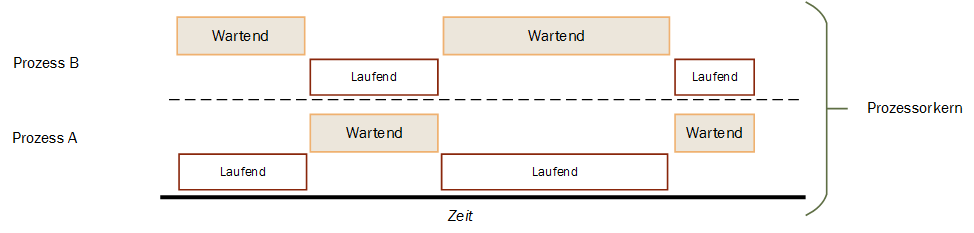
\includegraphics[width=0.7\linewidth]{images/time_slice}
	\caption{Multi-Programmierung\parencite[S. 128]{tanenbaum2016}}
	\label{fig:time_slice}
\end{figure}

Einige Arbeitsschritte eines Prozesses können direkt und ohne Verzögerung ausgeführt werden, andere Arbeitsschritte können durch den Zugriff auf langsame Ressourcen wie Festplatten I/O oder Kommunikation über Netzwerke zu Verzögerungen führen. In so einem Arbeitsschritt ist der Prozess blockiert und bis zur Erledigung des Zugriffs kann kein weiterer Arbeitsschritt ausgeführt werden. Das Betriebssystem markiert den Prozess nach dem Start der Anweisung als \emph{blockiert} und wechselt zu einem anderen Prozess. Ein Prozess kann dabei wie in \ref{fig:prozessstati} dargestellt mehrere Stati einnehmen. Er wird im Status Wartend angelegt, wird dann durch das Betriebssystem zur Ausführung ausgewählt und wird damit zum laufenden Prozess. Nach Ablauf der Zeitscheibe\footnote{Oder dem Aufruf einer Betriebssystemmethode wie \textit{yield} oder \textit{sleep} mit der ein thread anzeigen kann dass er nicht mehr weiter aktiv sein möchte} wird die Ausführung des Prozesses unterbrochen und er wird zum wartenden Prozess. Wird während der Ausführung eine Betriebssystemmethode ausgeführt die auf externe Ressourcen wartet dann wird der Prozess unterbrochen und bekommt den Status blockiert. Erst wenn die Betriebssystemmethode abgeschlossen wurde, wird der Prozess in den Status wartend überführt und kann somit wieder zur Ausführung ausgewählt werden.

\begin{figure}
	\centering
	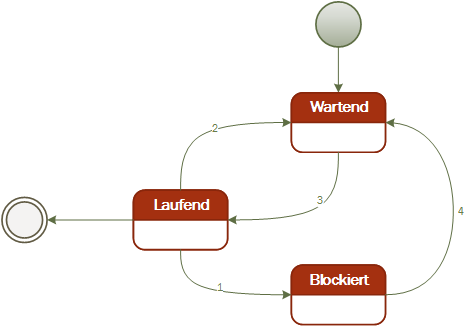
\includegraphics[width=0.7\linewidth]{images/pstates}
	\caption{Prozessstati\parencite[S. 134]{tanenbaum2016}\parencite[S. 152]{Dahlin2012}}
	\label{fig:prozessstati}
\end{figure}


Das Betriebssystem wechselt nur zu Prozessen die ausgeführt werden können. Gibt es zu einem Zeitpunkt viele Prozesse die blockiert sind\footnote{meist durch das Warten I/O auf Speichermedien} so ist die I/O Leistung des Rechners der die Leistung begrenzende Faktor, gibt es viele Prozesse die ausgeführt werden könnten ist es die Prozessorleistung.
\\Die lineare Ausführung der Anweisungen kann auch als \emph{thread of control} bezeichnet werden, womit jeder Prozess zumindest einen solchen \emph{thread} hat. Um innerhalb eines Prozesses mehrere Arbeiten gleichzeitig zu erledigen\footnote{Oder auch bestimmte Aufgaben wie I/O einfacher gestalten zu können} kann es wünschenswert sein, mehrere solche threads innerhalb des selben Prozesses, und damit innerhalb eines Adressraums zu verwenden. Dies kann innerhalb eines Prozesses durch die Erzeugung weiterer threads erfolgen. Ein Prozess kann praktisch eine beliebige Anzahl von threads gleichzeitig Anfordern\footnote{Unter Windows beschränkt meist durch den Hauptspeicher, unter Linux durch das Betriebssystem und einstellbar unter \textit{/proc/sys/kernel/threads-max}}. Aus praktischen Gründen sollte die tatsächlich angeforderte Anzahl deutlich darunter liegen, da sonst durch den nötigen Mehraufwand der Verwaltung innerhalb des Betriebssystems die positiven Effekte der Verwendung von threads wieder zunichte gemacht werden\footnote{"[The maximum thread count] doesn't matter, and if you find it does matter, you need to rethink what you're doing so that it doesn't matter"\parencite{stacko_threadcount}}.
\\Threads haben \parencite[S. 148]{tanenbaum2016}
\begin{itemize}
	\item einen eigenen Befehlszähler, es kann somit jeder thread unabhängig eine eigene Anweisung ausführen.
	\item einen eigenen Stack, und damit eine eigene Aufrufhierarchie und Argumente. für Funktionsaufrufe
	\item eigene Register.
	\item eigenen Zustand( siehe Prozesszustände).
	\item \emph{keinen} eigenen Adressraum, alle threads teilen sich die selben globalen Strukturen wie Dateien oder explizit allokiertem Speicher.
\end{itemize}	
Mit diesen Eigenschaften kann man einen Prozess also vereinfacht auch als einen thread mit Adressraum darstellen.\parencite[S. 1]{butenhof1997}
\subsection{Thread Programmierung}
Um threads nutzen zu können stellt das .NET Framework  Methoden zur Verfügung\parencite{ms_threading}\footnote{Die Funktionen um mit threads umzugehen folgen meist dem POSIX Thread Standard und sind somit in den meisten Betriebssystemen und Frameworks ähnlich\parencite{butenhof1997} }:
\begin{table}[]
	\centering
	\label{Ttab:thread-methoden}
	\begin{tabular}{| l | p{10cm} |}
		\hline
		\textit{\textbf{Methode}} & \textit{\textbf{Beschreibung}}  \\
		\hline
		new Thread()                                         &    Konstruktor mit dem ein neuer Thread angelegt, aber noch nicht gestartet wird\\
		\hline
		Thread.Start/(                                        &    Methode mit der der Thread gestartet wird und mit der Abarbeitung der Thread-Main Methode begonnen wird.\\
		\hline
		Thread.Abort()                                        &   Bricht die Ausführung eines Threads ab\\
		\hline
		Thread.Join()										 & Wartet auf die Beendigung eines Threads\\
		\hline
		Thread.Sleep()										& Unterbricht die Ausführung des Threads für eine bestimmte Zeitspanne\\
		\hline
		Thread.Yield()										& Gibt die Ausführung des aktuellen Threads auf und ermöglicht dem Betriebssystem einen neuen Thread auszuwählen\parencite{ms_threading_yield}\\
		\hline
	\end{tabular}
	\caption{.NET thread-Methoden}
\end{table}
Damit kann ein Prozess (und damit der erste thread innerhalb des Prozesses) weitere threads anlegen und diese wieder beenden. Ein einfaches Programm mit mehreren Threads in .NET/ C\# ist in Listing \ref{lst:thread_1} dargestellt.
\begin{lstlisting}[caption={Thread Hello World},label={lst:thread_1},captionpos=b]
class TestThread
{
	private volatile bool runThread = true;
	
	public void Main()
	{
		Thread threadMain = new Thread( ThreadMain );

		threadMain.Start();

		while ( threadMain.IsAlive ) ;

		Thread.Sleep( 10000 );

		runThread = false;
		threadMain.Join();
	}
	
	private void ThreadMain()
	{
		while( runThread )
		{
			Console.Out.WriteLine($"Thread {Thread.CurrentThread.Name} is here");
			Thread.Sleep( 1000 );
		}
	}
}
\end{lstlisting}
In Zeile 7 wird ein neuer Thread angelegt, aber noch nicht gestartet. Das Argument des Konstruktors ist die Methode die beim Starten des threads ausgeführt wird. In Zeile 9 wird der thread gestartet und ist ab diesem Zeitpunkt ausführbar. Die Ausführung startet nicht sofort, sondern dann wen das Betriebssystem den thread zur Ausführung auswählt. Aus diesem Grund wird in Zeile 11 darauf gewartet dass der Thread tatsächlich ausgeführt wurde\footnote{Genau genommen zumindest in einer Zeitscheibe ausgeführt wurde, er kann danach ja wieder unterbrochen werden.}\footnote{Würde man das \textit{Sleep} beginnen ohne dass der thread aktiv geworden ist, könnte die thread-run Variable auf false gesetzt werden, ohne dass der thread auch nur gestartet wurde. Der Zeitpunkt wann der Thread tatsächlich gestartet wird ist nicht vorhersagbar.}.
\\In Zeile 15 wird nach einiger Zeit dem thread mittels tread-run variable mitgeteilt dass er sich beenden soll. Damit kann der thread seine aktuelle Aufgabe beenden und sich danach beenden. Diese Variable muss als \emph{volatile} markiert sein, da sie sich außerhalb des aktuellen threads ändern kann und somit der Zugriff auf den Wert dieser Variable nicht durch Vorhersage der Instruktionen aus dem aktuellen thead vorhergesagt, und damit optimiert werden kann.\parencite{ms_volatile} Der thread könnte auch mithilfe von Thread.Abort() abgebrochen werden, dann wird er sofort abgebrochen ohne dass er eine eventuell gerade ausgeführte Aufgabe fertig abarbeiten kann. 
\\In Zeile 16 wird auf die Beendigung des threads gewartet und danach das Programm beendet.


\subsection{Synchronisierung}
Threads sind aus Sicht eines (Applikations-)Entwicklers virtualisierte Prozessorkerne. Der Entwickler kann vereinfacht annehmen dass die Hardware beliebig viele Prozessorkerne hat, die tatsächliche Zuteilung eines threads zur Ausführung auf einen Prozessorkern wird ihm durch das Betriebssystem abgenommen (Siehe Abbildung \ref{fig:threads_cores}). Diese Zuteilung erfolgt für alle threads über Prozessgrenzen hinweg und wird durch viele Parameter beeinflusst\footnote{Insgesamte Auslastung des Rechners, Prioritäten von Threads ...} und ist daher durch den Entwickler nicht vorherzusagen. Der Entwickler darf sich nicht auf eine gewisse Abfolge an Abläufen über mehrere threads hinweg verlassen. Ist eine definierte Reihenfolge notwendig, so muss diese durch den Entwickler explizit erzwungen werden. Die Anzahl an Prozessorkernen im Rechner ist die maximale Anzahl an gleichzeitig aktiven threads.\parencite[S. 140]{Dahlin2012}

\begin{figure}
	\centering
	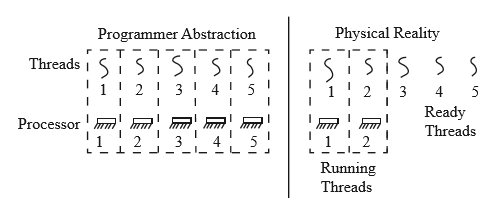
\includegraphics[width=0.7\linewidth]{images/threads_cores.png}
	\caption{Zuteilung threads zu Prozessorkernen\parencite[S. 140]{Dahlin2012}}
	\label{fig:threads_cores}
\end{figure}

In fast allen Anwendungszwecken haben threads Daten die nur durch sie selbst verändert werden. Diese werden als \emph{thread-local} oder \emph{per-thread} Daten genannt. Diese Daten können direkt manipuliert werden, da es zu keiner Beeinflussung durch andere threads kommen kann. Diese Daten werden entweder als Variablen am Stack angelegt oder in .NET innerhalb einer Klasse mittels der Hilfsklasse \textit{ThreadLocal} allokiert werden\parencite{ms_threadlocal}. 
\\Unglücklicherweise\footnote{Die Formulierung in \parencite[S. 179]{Dahlin2012} ist sehr treffend.} besteht aber meist die Notwendigkeit dass threads kooperieren und Daten gemeinsam nutzen müssen. Dies können nun globale Ergebnisdaten einer auf mehrere threads verteilten Berechnung sein oder auch Strukturen zur Verteilung von Arbeit (\textit{dispatching}) auf mehrere threads bei einer Trennung der Erzeugung von Arbeit (producer) und der Erledigung (consumer). Diese Zugriffe von mehreren threads auf dieselben Daten werden auch \emph{race-condition} genannt, da sich die threads ein Rennen liefern wer die Daten zuerst ändern kann.
\\Die einfachste race-condition ist in Codebeispiel \ref{lst:thread_2} dargestellt\parencite[S. 182]{Dahlin2012}. Am Ende des Programmes kann nicht mit Sicherheit gesagt werden, welchen Wert die Variable \textit{theValue} hat.

\begin{lstlisting}[caption={Thread race-condition},label={lst:thread_2},captionpos=b]
class TestRaceCondition
{
	private volatile Int32 theValue = 0;
	
	public void Main()
	{
        var thread1 = new Thread( () => theValue = 1 );
		var thread2 = new Thread( () => theValue = 42 );

		thread1.Start();
		thread2.Start();

		thread1.Join();
		thread2.Join();
	}
}
\end{lstlisting}

Solche nicht vorhersagbaren Zustände müssen vermieden werden. Ein erster, naiver Versuch ist in Codebeispiel \ref{lst:thread_3} dargestellt.\parencite[S. 180]{Dahlin2012}
\begin{lstlisting}[caption={Thread naiver Mutex},label={lst:thread_3},captionpos=b]
class TestNaiveMutex
{
    private volatile bool stepOneComplete = false;
	private volatile int valueOne = 0;
	private volatile int valueTwo = 0;

	public void Test_NaiveMutex()
	{
		var thread_1 = new Thread( () => {
			valueOne = 42;
			stepOneComplete = true;
		} );

		var thread_2 = new Thread( () => {
			while ( !stepOneComplete ) ;
			valueTwo = valueOne * 2;
		} );

	thread_1.Start(); thread_2.Start();
	thread_1.Join(); thread_2.Join();
}
\end{lstlisting}
Über die Variable \textit{stepOneComplete} wird versucht mit dem zweiten thread so lange zu warten (Zeile 15) bis das Ergebnis des ersten thread vorliegt. Das Problem ist hier nicht offensichtlich, da es erst durch das Kompilieren oder durch die CPU selbst entsteht. Alle modernen Compiler oder CPUs versuchen Code zu optimieren, und eine der Strategien dabei ist das Verschieben von Instruktionen ohne Seiteneffekte innerhalb \textit{eines} threads\parencite[S. 100]{ecma335}. Die Verschiebung der Zuweisung in Zeile 11 hätte in einem Programm mit nur einem thread keine Nebenwirkung, diese tritt erst durch den zweiten thread auf, und ist somit durch den Compiler oder die CPU nicht mehr erkennbar.
\\Die beiden obigen Beispiele haben schon in simplen Codebeispielen gezeigt, dass eine korrekte Umsetzung von Zugriffen auf geteilte Datenstrukturen unumgänglich ist. Dafür stehen Entwicklern folgende Methoden zur Verfügung\parencite[S. 170ff]{tanenbaum2016}:
\begin{itemize}
	\item Vermeiden von gemeinsamen Datenstrukturen
	\item Atomare Operationen
	\item Speicherbarrieren
	\item Sperren
	\item Monitore
\end{itemize}
\subsubsection{Vermeiden von gemeinsamen Datenstrukturen}	
Das Vermeiden von gemeinsam genutzten Datenstrukturen ist der sicherste und effizienteste Weg um sich vor race-conditions zu schützen. Bei komplexen Aufgaben kann die Stabilität und Ausführungsgeschwindigkeit drastisch erhöht werden wenn die verwendeten Algorithmen - wo möglich - geändert werden, so dass kein Zugriff auf gemeinsame Datenstrukturen notwendig ist. Auch eine Reduktion der Häufigkeit der Zugriffe auf gemeinsam genutzte Datenstrukturen ist hilfreich. So könnten in etwa Ergebnisse innerhalb eines threads berechnet werden und erst am Ende einmalig mit dem Gesamtergebnis zusammengeführt werden, anstatt Ergebnisse einzelner Rechenschritte in ein Gesamtergebnis zu speichern.
\\Diese nicht-globalen Daten können
\begin{enumerate}
	\item in der thread-main Methode allokiert werden und sind damit am Stack der pro thread angelegt wird.
	\item oder als \textit{thread specifc data} deklariert werden. Damit werden diese Datenstrukturen durch die .NET-Runtime für jeden thread extra angelegt.
\end{enumerate}

\subsubsection{Atomare Operationen}	
Eine atomare Operation ist eine Anweisung die durch die CPU ausgeführt wird und in einem Schritt ohne Unterbrechung durchgeführt wird. Diese Operationen beziehen sich auf Datentype mit der Größe der \textit{native word size} des Prozessors\parencite[S. 102]{ecma335}, derzeit in der Regel 64bit. In Codebeispiel \ref{lst:thread_2}  in etwa ist der Wert von \textit{theValue} immer 1 oder 42, aber niemals etwas anderes. Würde der Datentyp in etwa \textit{double}\footnote{Double hat eine Länge von 64 bit} sein, ist die Größe des Datentyps nicht mehr atomar, die einfache Zuweisung \textit{theValue = 42;} ist nicht mehr garantiert ohne Unterbrechung durchgeführt zu werden. Somit könnte der erste thread den ersten Teil des Wertes schreiben, dann unterbrochen werden, der zweite thread die Variable setzen, und danach der erste thread den zweiten Teil des Wertes schreiben. Damit ist der Inhalt von \textit{theValue} nicht vorhersagbar. Atomare Operationen sind vor allem für leistungsorientierte Entwicklung wichtig, da sie einen korrekten Zugriff auf zwischen threads geteilte Ressourcen garantieren ohne dass Sperren verwendet werden müssen.
\\In .Net gibt es die eigene Klasse \textit{Interlocked}die mehrere Methoden zur Verfügung stellt die garantiert unterbrechungsfrei sind. Da .Net auf mehreren Plattformen zur Verfügung steht sind diese entweder mittels atomarer Operationen oder mittels Sperren implementiert.

\subsubsection{Speicherbarrieren}
Eine Speicherbarriere ist eine Anweisung an den Compiler und die CPU keine Ablaufoptimierung durch verschieben von Instruktionen über die Barriere hinweg durchzuführen. Es wird also garantiert dass alle Anweisungen vor der Barriere von der CPU tatsächlich vor allen anderen Anweisungen nach der Barriere ausgeführt werden.\parencite[S. 195]{tanenbaum2016} Damit kann das in Codebeispiel \ref{lst:thread_3} angeführte Problem behoben werden. In C\# wird eine Speicherbarriere durch den Aufruf von \textit{Interlocked.MemoryBarrier()} realisiert.\parencite{ms_interlocked_barrier}\footnote{Siehe auch \textit{NaiveMutexBarrier.cs}}

\subsubsection{Sperren}\label{sss:Sperren}	
Sperren (locks) bieten eine Möglichkeit sicherzustellen dass nur ein thread innerhalb eines bestimmten Abschnittes des Codes aktiv sein kann. Die Ausführung aller Anweisungen innerhalb des mit einer Sperre geschützten Bereiches wirken auf alle anderen threads \textit{atomar} da immer alle Anweisungen ausgeführt werden bevor ein anderer thread den Code-Block ausführen kann. Dadurch können Veränderungen an Datentypen die nicht atomar sind durchgeführt werden und ein konsistenter Zustand der Daten garantiert werden. 
\\Die Ausführung von Code innerhalb einer Sperre kann natürlich weiterhin unterbrochen werden und zu einem späteren Zeitpunkt fortgesetzt wird. Versucht ein anderer thread die selbe Sperre für sich zu allokieren, wird der thread unterbrochen und in den Status blockiert gesetzt. Erst wenn die Sperre durch den ersten thread freigegeben wird, setzt das Betriebssystem den thread in den Status wartend. Dadurch steht er für die Ausführung innerhalb einer der nächsten Zeitscheiben bereit. Auch hier gilt, dass der zweite thread nicht sofort nach frei werden der Sperre ausgeführt wird, sondern zu einem beliebigem Zeitpunkt.

\subsubsection{Monitore}	
Mit den bisher vorgestellten Techniken kann ein Programm mit mehreren threads korrekt, also ohne unbeabsichtigte Seiteneffekte durch Manipulation von globalen Daten\footnote{Daten die für mehrere threads sichtbar sind.}  implementiert werden. 
\\Monitore\footnote{Oder auch \textit{condition} genannt\parencite[S. 199]{Dahlin2012}.} bieten die Möglichkeit, dass ein thread auf einen anderen thread wartet. Dies wird in benötigt, wenn ein thread für die Abhandlung der Kommunikation zuständig ist (der sogenannte Erzeuger), und ein anderer thread die Abarbeitung der übermittelten Dateninhalte durchführt (der so genannte Verbraucher). Nur mit den bisher vorgestellten Methoden ist dies nur mittels \textit{polling}, einem ständigen Nachfragen durch den zweiten thread, möglich\footnote{Dies wird Erzeuger-Verbraucher (producer-consumer) Problem genannt\parencite[S. 188]{tanenbaum2016}}\parencite[S. 199ff]{Dahlin2012}. 
\begin{lstlisting}[caption={Thread naiver Monitor},label={lst:thread_busywait},captionpos=b]
public T DequeBusy()
{
	bool dequeSuccess = false;
	T result = default( T );

	while ( !dequeSuccess )
	{
		lock ( myLock )
		{
			if( backingStore.Any() )
			{
				dequeSuccess = true;
				return backingStore.Dequeue();
			}
		}
	}
}

\end{lstlisting}
Diese Implementierung, wie in Codebeispiel \ref{lst:thread_busywait} dargestellt, hat den gravierenden Nachteil dass der thread Rechenleistung verbraucht ohne tatsächliche Arbeit zu verrichten. Dies geschieht durch die Schleife in Zeile 6, die erst verlassen wird wenn tatsächlich wieder Arbeit vorhanden ist. Damit kann dieser eine thread sogar die Ausführung der weiteren threads, also auch des threads der die Arbeit erzeugt, verlangsamen. Das Hinzufügen eines \textit{sleep} Befehls oder eines erzwungenen thread-Wechsel mittels \textit{yield} mildert zwar das Problem der CPU-Belastung, jedoch führen beide Instruktionen zu einem Overhead da die threads in kurzer Zeit gewechselt werden müssen, was auch zu einer hohen CPU Beanspruchung führt.
\\Monitore bieten nun die Möglichkeit zusammen mit Sperren dies zu lösen. Dazu stellen sie folgende Methoden zur Verfügung:\parencite[S. 201]{Dahlin2012}\parencite{ms_monitor}
\begin{itemize}
	\item \textit{Wait()} - Gibt in einem atomaren Schritt die verbundene Sperre frei und versetzt den thread in den Status blockiert. Damit wird der thread nicht weiter ausgeführt und verbraucht keine CPU-Ressourcen mehr. Der thread wird in der Monitor-Variable als auf diese wartend eingetragen\footnote{in .Net ist dies die Sperrvariable.}. Vor der Rückkehr aus der Methode wird die Sperre wieder gesetzt.
	\item \textit{Signal()} (in .Net \textit{Pulse()} genannt) - Setzt einen der auf diese Monitor -Variable wartenden threads in den Zustand Wartend, damit wird er gemäß dem Scheduling ausgeführt\footnote{Die Ausführung beginnt nicht sofort, der Zeitpunkt ist abhängig von der Last im System}.
	\item \textit{Broadcast()} (in .Net \textit{PulseAll()} genannt) - Setzt alle threads die auf diese Monitor-Variable warten in den Zustand Wartend. Damit werden alle diese threads ausgeführt.
\end{itemize}
 Damit kann das Codebeispiel \ref{lst:thread_busywait} nun korrekt umgesetzt werden, wie in Codebeispiel\ref{lst:thread_deq} dargestellt.
\begin{lstlisting}[caption={Thread Monitor.Wait()},label={lst:thread_deq},captionpos=b]
public T Dequeue()
{
	lock( myLock )
	{

		while ( ! backingStore.Any() )
		{
			Monitor.Wait( myLock );
		}

		return backingStore.Dequeue();
	}
}
\end{lstlisting}
In Zeile 8 wird der thread solange unterbrochen bis der Monitor von einem anderen thread signalisiert wird. Die Sperre ist vor dem Eintritt in das Wait() gesetzt. Die Schleife in Zeile 6 hat mehrere Aufgaben. Wenn schon Arbeit existiert, wird diese ohne weiteres Wait() abgearbeitet. Dies ist notwendig, da ein vorhergehendes \textit{Pulse} nicht auf der Monitor-Variable vermerkt wird. Würde also Wait() ohne Prüfung aufgerufen werden, so würde der thread unterbrochen werden obwohl Arbeit vorhanden wäre. Desweiteren wird nachdem \textit{Wait()} verlassen wird wieder geprüft ob tatsächlich Arbeit vorhanden ist. Dies ist notwendig, denn wenn es mehrere Verbraucher gibt kann die von einem anderen thread erzeugte Arbeit bereits durch einen anderen thread abgearbeitet sein. Der dann durch das \textit{Pulse()} aufgeweckte thread findet dann keine weitere Arbeit mehr vor. Dies ist in Ablaufdiagram \ref{fig:threads_pcs} dargestellt.

\begin{figure}
	\centering
	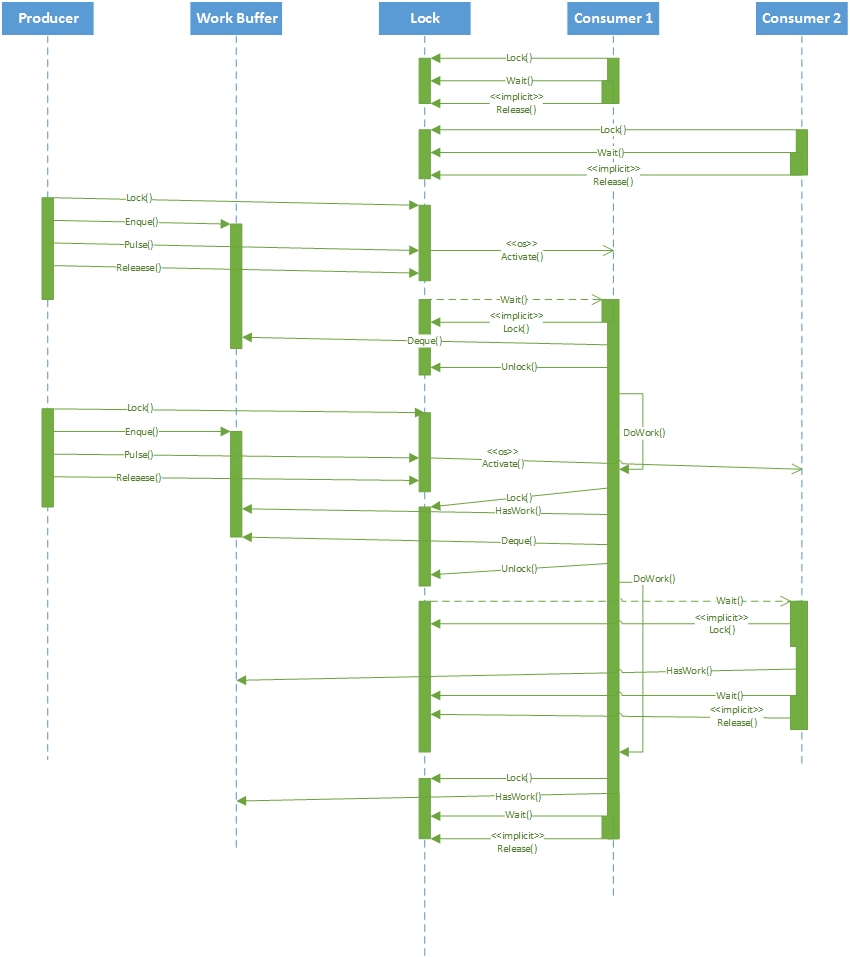
\includegraphics[width=0.9\linewidth]{images/uml-sequence_pulse.png}
	\caption{Erzeuger/ Verbraucher Modell - Ablauf \parencite[S. 405]{posa2} }
	\label{fig:threads_pcs}
\end{figure}

Der Erzeuger ist in Codebeispiel \ref{lst:thread_enq} dargestellt. Nachdem die Sperre gesetzt wird, wird die neue Arbeit in Zeile 5 eingetragen und in Zeile 7 wird die Monitor-Variable ausgelöst, was zu einer - zeitlich verzögerten - Aktivierung eines Verbraucher-threads führt. Die Sperre wird während des Aufrufes von \textit{Pulse()} nicht modifiziert, sie bleibt erhalten.
\begin{lstlisting}[caption={Thread Monitor.Pulse()},label={lst:thread_enq},captionpos=b]
public void Enque( T newElement )
{
	lock( myLock )
	{
		backingStore.Enqueue( newElement );

		Monitor.Pulse( myLock );
	}
}
\end{lstlisting}
\subsection{Zusammenfassung}
Threads stellen eine wichtigen Baustein der Programmierung dar, vor allem wen es darum geht performante Programme zu entwickeln die komplexe Aufgabenstellungen zu bewältigen haben. Threads werden oft von eingesetzten Frameworks verwendet und vom Entwickler versteckt, daher ist ein Grundwissen für alle Entwickler notwendig. 
\\Die essentiellen Punkte wenn es um Concurrency geht sind
\begin{itemize}
	\item sich dessen bewusst zu sein welche Daten global, also für mehrere threads sichtbar sind, und wie diese zu schützen sind. 
	\item sich bewusst zu sein, dass es keine Garantien für Zeitpunkte gibt. Jeder thread kann zu jedem Zeitpunkt, auch innerhalb einer Sperre, unterbrochen werden und erst zu einem späteren, nicht vorhersehbarem Zeitpunkt fortgesetzt werden.
	\item zu wissen, das das Starten oder Aufwecken eines threads nicht sofort erfolgt, sonder auch erst zu einem späterem, durch das Betriebssystem festgelegten Zeitpunkt.
\end{itemize}


\section{Relationale Datenbanken}
Datenbanken sind Systeme in denen große Datenmengen effizient gespeichert und verwaltet werden können. Dabei wird vom System eine Schnittstelle zur Verfügung gestellt die das Arbeiten mit den Daten ohne Wissen über deren tatsächliche Speicherung ermöglicht. Die Daten innerhalb des Systems werden in einem \emph{Modell} beschrieben, das die Komplexität der physischen Speicherung nicht darstellt. Diese bleibt dem System selbst überlassen und wird von diesem bei den meisten modernen Systemen dynamisch ausgewählt um für die jeweiligen Daten und die Art der Zugriffe auf diese eine optimale Leistung zur Verfügung zu stellen.
\\Bei relationalen Datenbanken werden die Informationen nach thematischer Zusammengehörigkeit in so genanten Tabellen gespeichert.\footnote{\emph{Relational} wird in seiner mathematischen Bedeutung verwendet.} Diese Art von Datenbanken wurde erstmals von Edgar F. Codd vorgestellt und galt bis vor wenigen Jahren als alleiniger Standard für Datenbanken. \parencite[S. 133]{dbgrund}. Erst durch die immensen Datenmengen der Big-Data wurde für diese Anwendung die so genannten \emph{No-SQL}\footnote{\emph{N}ot \emph{O}nly \emph{SQL}, diese Datenbanken stellen weitere Formen der Speicherung wie schemenlose Dokument-Datenbanken, Wertepaare oder Graphdatenbanken zur Verfügung. \parencite[S. 11ff]{Fasel2016} } Datenbanken eingeführt. Bei diesen werden einige der unten Beschriebenen strengen Regeln der Datenstruktur und Datenkonsistenz aufgehoben um eine höhere Leistung zu erreichen.
\\Bei relationalen Datenbanken werden thematisch Zusammengehörige Daten in einer Tabelle gespeichert. Jede Datenbank umfasst mehrerer solcher Tabellen. Jede Tabelle enthält Datensätze, so genannte \emph{Tupel}. Jeder dieser Tupel besteht aus immer den selben \emph{Attributen}, die beschreiben welche Daten die Tabelle enthält. Tabellen sind also eine Zusammensetzung aus der Beschreibung der Struktur der Daten und den Daten selbst. Die Beschreibung der Struktur der Daten wird auch \emph{Schema} oder \emph{Katalog} genannt.
\\Ein Beispiel für eine Tabelle ist die Tabelle 'Student', die die Attribute Vorname, Nachname, Matrikelnummer und Geburtsjahr enthält. Ein Datensatz darin ist dann zum Beispiel 'Max', 'Mustermann', '4711', '1980'.\parencite[S. 137]{dbgrund} \parencite{DBLP:journals/cacm/Codd70}
\\Die von Codd vorgeschlagene Trennung in Benutzersicht und Speicherung hat nun den Vorteil dass der Student (Vorname: 'Max', Nachname: 'Mustermann') durch Änderung der Beschreibung der Sicht auch als Student( Nachname: 'Mustermann', Geburtsjahr: '1980') dargestellt werden kann.\footnote{Dies wird auch \emph{Projektion} genannt, eine Änderung der Darstellung ohne Änderung der zugrundeliegenden Daten\parencite[S. 152]{dbgrund} }
\\Bei relationalen Datenbanken hat sich als Standard für die Manipulation des Schemas und der Daten die SQL\footnote{\emph{S}tructured \emph{[Q}uery \emph{L}anguage, genormt nach der ISO/ IEC 19075 Standard-Familie der von allen relationalen Datenbanksystemen unterstützt wird\parencite{ocl_sql}\parencite{isosql}\footnote{Jeweils mit eigenen, unterschiedlich mächtigen Erweiterungen um den Anwendungsentwicklern einen Austausch des zugrundeliegenden Systems zu erschweren}} etabliert. Mit deren Hilfe können\parencite[S. 182]{dbgrund}
\begin{itemize}
	\item Schemata verwaltet werden. Dieser Teil der Sprache wird auch \emph{Data Manipulation Language (DML)} genannt. Er enthält Befehle um 
	\begin{itemize}
		\item Tabellen anzulegen
		\item Tabellen zu modifizieren
		\item Tabellen zu löschen und
		\item Beschränkungen anzulegen und zu löschen.
	\end{itemize}
	\item Daten verwaltet werden. Dieser Teil der Teil der Sprache wird auch \emph{Data Definition Language (DDL)} genannt. Er enthält Befehle um
	\begin{itemize}
		\item Datensätze anzulegen
		\item Datensätze auszulesen
		\item Datensätze zu modifizieren und
		\item Datensätze zu löschen.
	\end{itemize}
\end{itemize} werden.
Zusätzlich zu dieser Standardisierung des Zugriffes bieten relationale Datenbanksysteme weitere Garantien die das Arbeiten mit großen Datenmengen vereinfachen. Diese Garantien beziehen sich auf Veränderungen von Daten die in so genannten \emph{Transaktionen} durchgeführt werden. Eine Transaktion beinhält dabei alle Veränderungen an Daten die als Einheit durchgeführt werden sollen. Entweder werden alle Veränderungen erfolgreich durchgeführt, oder aber keine einzige der Veränderungen innerhalb einer Transaktion wird durchgeführt. Diese Garantien werden auch als \emph{ACID} bezeichnet:\parencite[S. 6fs]{GrayReuter93}\parencite[S. 23ff]{WeikumVossen02}
\begin{itemize}
	\item \emph{Atomic} (Atomar) - Die Veränderungen die eine Transaktion am Datenbestand durchführt sind atomar, sie werden also alle durchgeführt oder keine der Veränderungen findet statt.
	\item \emph{Consistent} (Konsistent) - Die Transaktion ist eine innerhalb der im Schema definierten Regeln gültige Veränderung der Daten. Die Daten sind am Ende der Transaktion in einem gültigen und konsistenten Zustand. Die Anwendung muss dafür sorgen, dass die Daten so verändert werden, dass dieser Zustand erreicht werden kann. Bei einem Fremdschlüssel muss der referenzierte Datensatz zuvor eingetragen worden sein.\footnote{Das Datenbanksystem würde nur das Speichern des referenzierenden Datensatzes verhindern, es kann weder den Datensatz erzeugen noch die Reihenfolgen des Einfügens ändern.}
	\item \emph{Isolated} (Isoliert) - Transaktionen laufen unabhängig voneinander ab, obwohl sie zeitgleich laufen können. Eine zweite Transaktion findet entweder komplett vor oder komplett nach einer Transaktion statt.
	\item \emph{Durable} (Dauerhaft) - Wenn eine Transaktion erfolgreich abgeschlossen wurde, ist die Veränderung dauerhaft gespeichert, auch wenn es danach zu Fehlern oder Abstürzen kommt.
\end{itemize}
Die Grenzen der Transaktion, also deren Beginn und Ende wird durch das Anwendungsprogramm festgelegt. Das Anwendungsprogramm kann am Ende der Transaktion die Änderungen speichern (\emph{commit}) oder die Änderungen bewusst verwerfen (\emph{rollback}).
\subsection{Sperren}
Um die oben angeführten \emph{ACID} Eigenschaften sicherzustellen auch wenn mehrere Benutzer, oder generalisiert, mehrere Transaktionen gleichzeitig Daten verändern, müssen diese die Daten wie auch in Kapitel \ref{sss:Sperren} beschreiben geschützt werden. Dafür stellen Datenbanksysteme einige Konzepte und Funktionen zur Verfügung:
\begin{itemize}
	\item Sperren der gesamten Datenbank - Damit kann nur mehr eine Transaktion die Daten und das Schema in der Datenbank verändern. Aufgrund der großen Auswirkung werdend solche Sperren praktisch nur beim Nieder- und Hochfahren des Systems verwendet. Ein explizites setzen solcher Sperren aus einer Anwendung heraus ist nicht nötig.
	\item Sperren auf Tabellenebene - Damit kann nur mehr eine Transaktion die Daten in einer Tabelle verändern. Aufgrund der großen Auswirkungen im System wird diese Art der Sperre durch eine Transaktion mittlerweile nicht mehr unterstützt. Innerhalb des Datenbanksystems werden solche Sperren dann genutzt wenn in etwa das Schema der Tabelle, also ihre Struktur geändert wird. Auch die Neuberechnung oder Reorganisation von Indizes kann eine Sperre auf Tabellenebene auslösen.\parencite{ms_idx_rebuild}
	\item Sperren auf Seiten- oder Block-Ebene - Seiten sind Konstrukte innerhalb des Datenbanksystems welche eine Menge von Datensätzen bündeln die in einer Einheit auf den Datenträger gespeichert werden. Die Seiten können nochmals zu größeren Einheiten, den Blöcken zusammengefasst werden.\footnote{Die Historisierung und damit die kontrollierte Veränderung der Daten wird von den meisten Datenbanksysteme ebenfalls über diese Einheiten abgebildet. Wenn es neuere Daten gibt, so wird - stark vereinfacht - der Block kopiert, die Daten in der Kopie aktualisiert und zuletzt ein Verweis im bisherigen Block auf den neuen Block gesetzt.}\parencite[S. 30f]{WeikumVossen02} Da immer die gesamte Einheit gelesen und geschrieben wird, ist eine Sperre auf eine solche Einheit für das Datenbanksystem sehr effizient durchzuführen. Ist so eine Sperre gesetzt, kann nur mehr eine Transaktion eine Veränderung an allen Datensätzen in dieser Einheit durchführen.
	\item Sperren auf Datensatzebene - Es kann nur mehr eine Transaktion die Inhalte eines Datensatzes ändern. Dies ist in der Regel die feinste Granularität an Sperren die ein Datenbanksystem bietet.
	\item Optimistische Sperren - Beim optimistischem Sperren handelt es sich nicht um eine Sperre die innerhalb der Datenbank umgesetzt wird, sondern um eine Methodik die in Anwendungsprogrammen umgesetzt werden muss. Dabei werden die Daten ohne Sperre gelesen und verarbeitet. Beim Schreiben von Änderungen erst wird der Datensatz gesperrt und die Inhalte aktualisiert. Dadurch wird die Dauer in der der Datensatz gesperrt ist auf das bloße Schreiben der Änderungen beschränkt. Um sicherzustellen dass keine Änderungen in der Zwischenzeit vorgenommen wurden, muss beim Aktualisieren nicht nur der Schlüssel des Datensatzes, sondern auch eine \emph{Identität}. Diese wird bei jeder Änderung verändert\footnote{meist ein Zähler der Inkrementiert wird}, dadurch kann der Datensatz nur verändert werden wenn sich der Inhalt nicht verändert hat. Das Anwendungsprogramm muss allerdings ein Scheitern des Updates behandeln.\parencite[S. 366]{WeikumVossen02}
	\begin{figure}
		\centering
		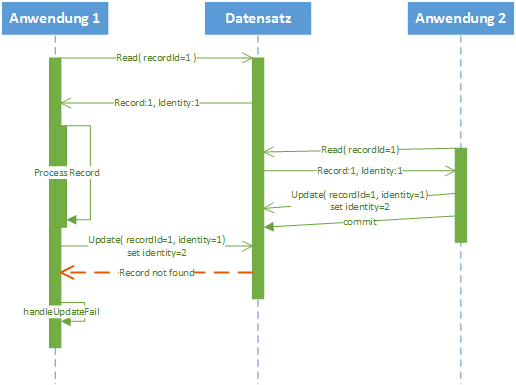
\includegraphics[width=0.7\linewidth]{images/optimistic_lock.png}
		\caption{Ablauf optimistische Sperren, eigene Darstellung}
		\label{fig:optimistic_locking}
	\end{figure}
\end{itemize}
Die Granularität der Sperre wird in der Regel durch das Datenbanksystem festgelegt und im Verlauf der Transaktion wenn nötig angepasst. Eine Transaktion kann zum Beispiel mit einer Datensatzsperre beginnen, wenn im Verlauf der Transaktion mehrere aufeinanderfolgende Datensätze geändert werden wird die Sperre auf eine Seiten- oder Block-Sperre erweitert.\parencite[S. 366f]{WeikumVossen02}
\\Wenn eine zweite Transaktion Datensätze ändern will die gesperrt sind, so wird diese Transaktion blockiert, solange bis die Sperre gesetzt werden kann - frühestens also dann wenn die Sperre von der ersten Transaktion aufgehoben wird. Werden nun zwei Datensätze, Satz A und B gesperrt, und von einer zweiten Transaktion die gleichen Datensätze, allerdings in der Reihenfolge B,A kann es zu einem \emph{Deadlock} kommen. In der ersten Zeitscheibe wird von der ersten Transaktion Datensatz A und von der zweiten Datensatz B gesperrt. In der darauffolgenden Zeitscheibe versucht nun die erste Transaktion B zu sperren und wird blockiert, die zweite Transaktion versucht A zu sperren und wird blockiert. Beide Transaktionen sind nun blockiert und können nicht mehr fortgesetzt werden da die Ressourcen kreuzweise gesperrt sind und  durch die Blockade beider Transaktionen nicht mehr freigegeben werden.\parencite[S. 138]{WeikumVossen02}
\\Die einfachste Methode dies aufzulösen ist dass die Transaktion die am längsten blockiert nach Ablauf einer definierten Zeit abgebrochen wird. Dadurch wird die Sperre auf Datensatz A aufgehoben und die zweite Transaktion kann erfolgreich beendet werden.\parencite[S. 139ff]{WeikumVossen02}
\\Um Deadlocks von vorne herein zu Vermeiden sollten Ressourcen immer in der selben Reihenfolge allokiert werden. Die zweite Transkation könnte dann schon Datensatz A nicht sperren, würde blockieren und die ersten Transaktion könnte vollständig abgearbeitet werden wodurch die zweite dann ebenso durchlaufen kann.


\subsection{Probleme durch mehrere Transaktionen}\label{subs:isolation}
Beim gleichzeitigen Lesen und Schreiben von Daten durch mehrere Transaktionen kann es zu vier grundlegenden Problemen kommen:
\begin{itemize}
	\item \emph{Lost Update} - bei einem Lost Update lesen zwei Transaktionen einen Datensatz, verändern den Inhalt eines Feldes und schreiben den Datensatz zurück. Die Änderung die dabei zuletzt durchgeführt wurde bleibt bestehen, die Änderung durch frühere Transaktion geht dabei verloren. Dies kann in etwa vorkommen wenn ein Datensatz einem Benutzer angezeigt wird und dieser danach eine Änderung vornimmt und speichert. Der Datensatz ist dabei in der Regel nicht mehr von der Datenbank gesperrt und daher nicht durch grundlegende Mechanismen geschützt. Wenn nun beim Speichern nicht geprüft wird ob der Datensatz in der Datenbank verändert wurde, so gehen Änderungen durch andere Benutzer oder Systeme die in der Zeit seit dem Laden des Datensatzes vorgenommen wurden, verloren.\parencite[S. 415f]{dbgrund}
	\item \emph{Dirty Read} - Dabei wird durch eine Transaktion T1 eine Änderung an einem Datensatz durchgeführt, aber noch nicht commited. Eine Transaktion T2 liest nun den schon geänderten Wert und danach wird Transaktion T1 abgebrochen. Damit hat T2 einen Wert in einem Datensatz gelesen der nicht commited war. In der Regel wird dies durch Datenbanksysteme verhindert, jedoch kann man dies zur Leistungssteigerung bewusst umgehen. Damit muss ein dirty read in der Programmlogik abgefangen werden.\parencite[S. 439]{dbgrund}
	\item \emph{Unrepeatable Read} - Wenn eine Transaktion einen Datensatz liest, kann eine andere Transaktion den gelesenen Datensätze verändern und committen. Führt nun die erste Transaktion die Abfrage erneut aus, so erhält sie andere Werte innerhalb des Datensatzes. Das Lesen ist damit nicht garantiert wiederholbar.\parencite[S. 439]{dbgrund}
	\item \emph{Phantom Read} - Wenn eine Transaktion eine Abfrage ausführt die Bedingungen enthält, so kann eine andere Transaktion Datensätze einfügen die der Abfrage enstprechen. Führt die erste Transaktion die Abfrage erneut aus, so erhält sie nun Datensätze die zuerst nicht enthalten waren, so genannte Phantome.\parencite[S. 439]{dbgrund}	
\end{itemize}
Die Lösung auf die letzen drei Probleme ist in den meisten relationalen Datenbanken Standard und kann über die Nutzung der \emph{Isolationstufen} gesteuert werden. Im SQL Standard sind folgende vier Isolationsstufen definiert:
\begin{table}[]
	\centering
\begin{tabular}{|l|c|c|c|}
	\hline 
	\textbf{Isolationsstufe}& \textit{Dirty Read} & \textit{Unrepeatable Read} & \textit{Phantom Read} \\ 
	\hline 
	\textit{READ UNCOMMITED}& Ja & Ja & Ja \\ 
	\hline 
	\textit{READ COMMITED}& Nein & Ja  & Ja \\ 
	\hline 
	\textit{REPEATABLE READ}& Nein & Nein & Ja \\ 
	\hline 
	\textit{SERIALIZABLE}& Nein & Nein & Nein \\ 
	\hline 
\end{tabular} 
\caption{Standard SQL Isolationsstufen, siehe \parencite[S. 440]{dbgrund}}
\label{table:isolationlevel}
\end {table}
Tabelle \ref{table:isolationlevel} zeigt die vier Isolationsstufen und die Probleme die sie vermeiden. Mit diesen Isolationsstufen kann eine grundlegende Funktion bei nebenläufigen Anwendungen schon auf Ebene des Datenbanksystems sichergestellt werden und muss somit nicht mehr in den einzelnen Applikationen abgehandelt werden. Besteht aber dennoch der Bedarf eine andere Isolationsstufe zu verwenden, so kann für eine Transaktion diese geändert werden.\footnote{Beim verwendeten SQL Server ist die Standard Isolationsstufe READ COMMITED\parencite{ms_isolation}}
\chapterend

  \selectlanguage{german}
%-----------------------------------------------------------------------------
\chapter{Umsetzung}\label{chap:Umsetzung}
%-----------------------------------------------------------------------------
\chapterstart
In diesem Kapitel wird die Umsetzung der Anforderungen in die Software erläutert. Es werden dabei besonders die Aspekte der Datenpersistenz, der Concurrency und der Skalierbarkeit vorgestellt.
\section{Überblick und Architektur}
Ausgehend von den Anforderungen wurde die Umsetzung des Schedulers\footnote{Die Umsetzung erfolgte unter dem Namen \textit{dJob}.} in Verantwortlichkeiten geteilt:
\begin{enumerate}
	\item Die Start-Prozedur
	\item Die \textit{Worker} die die Umsetzung der Aufgaben übernehmen
	\item Das Ausführen der Aufgaben \textit{Job} und planen der nächsten Ausführungszeit - der \textit{Scheduler}
	\item Das Laden von Aufgaben - der \textit{JobLoader}
\end{enumerate}
Die Trennung der Umsetzung erfolgte für den Scheduler und den JobLoader durch Interfaces gekapselt (siehe \ref{fig:architecture}). Die Instanziierung der tatsächlichen Klassen erfolgt zur Laufzeit über \textit{dependency injection}\cite{fowler2004}. Damit können diese Teile ausgetauscht werden und in etwa der Scheduler durch einen Echtzeit-fähigen Scheduler ausgetauscht werden ohne am Code selbst etwas ändern zu müssen\footnote{Die Umsetzung der injection dependency erfolgt in der Klasse \textit{ObjectRepository} ebenso um Rahmen dieser Arbeit. Umgesetzt wurde eine von außen konfigurierbare, explizite injection, einem \textit{service locator} nach Fowler. Verwendet wird diese mittels \code{var service = ObjectRepository.Get<ServiceType().}}.
\begin{figure}
	\centering
	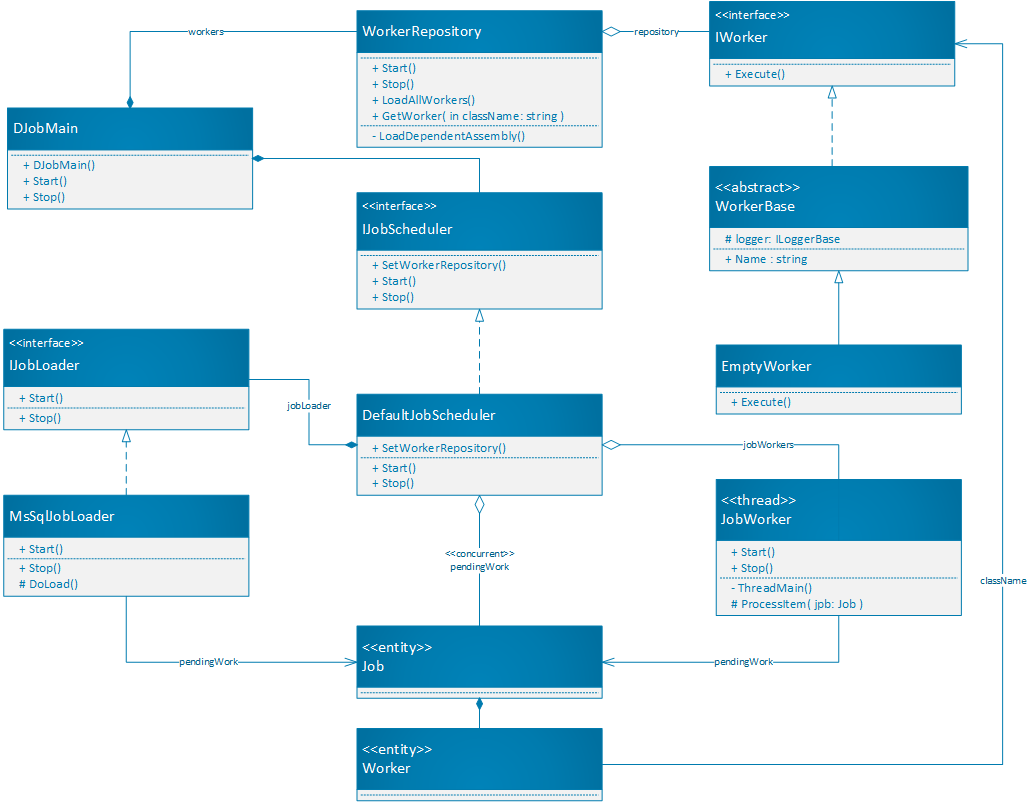
\includegraphics[width=0.7\linewidth]{images/architecture.png}
	\caption{Architekturübersicht des Schedulers, eigene Darstellung}
	\label{fig:architecture}
\end{figure}
Nach dem Start und der Initialisierung werden die Tasks die als nächstes ausgeführt werden sollen durch den JobLoader geladen und für andere Instanzen gesperrt. Dies geschieht durch das setzen des aktuellen Servers im Job (\code{Job.AllocatedTo}). Damit werden diese Jobs von anderen Instanzen ignoriert. Die Jobs werden dann in die interne Warteschlange (\code{pendingWork}) eingetragen.
\\Die Jobs in der Warteschlange werden durch die einzelnen Threads abgeholt, verarbeitet und die Job-Daten inklusiver dem Zeitpunkt der nächsten Ausführung in der Datenbank aktualisiert.
\\Die Verarbeitung selbst wird durch die Implementation des \code{IWorker} der für den Job vorgesehen ist (\code{Job.Worker}) erledigt. Welche Arbeiten verrichtet werden ist dem System nicht bekannt. Diese Worker werden durch den Klassennamen identifiziert und beim Starten des Systems aus dynamischen Bibliotheken geladen und instantiiert (siehe Kapitel \ref{sec:dynload}). Diese Entkopplung entspricht dem \emph{Command Pattern} \parencite{gamma1995}. Der \code{JobWorker} nimmt die Rolle des Receivers und des Clients gleichzeitig ein, da er vor der Ausführung noch das gewünschte ConcreteCommand aussucht.

\section{Datenbank}
Die Datenbank dient zur Speicherung aller notwendigen Daten. Es werden - ausgenommen Ablaufprotokolle - keine Daten anderswo gespeichert. Damit sind die Informationen zu den Jobs und zu deren Ausführungen zentral für alle Benutzer einsehbar und es können auch die Zugriffsrechte für Benutzer an einer Stelle gesteuert werden. Weiters werden Techniken die die Datenbank bereitstellt genutzt um eine Skalierung zu unterstützen (siehe Kapitel \ref{sec:scaling}).
\subsection{Datenbankmodell}
Das Datenbankmodell ist simpel gehalten und entspricht der \emph{dritten Normalform}. Es gibt also (vgl. \parencite[S. 317ff]{dbgrund})\begin{itemize}
	\item keine Felder die mehrere Werte enthalten (erste Normalform),
	\item keine Felder die die selbe Art von Werten enthalten (zweite Normalform)\footnote{Also in etwa die Felder Ausführungszeitpunkt1, Ausführungszeitpunkt2 ...}
	\item keine Wiederholungen von nicht-Schlüsselwerten in mehreren Datensätzen (dritte Normalform)
\end{itemize}
\begin{figure}
	\centering
	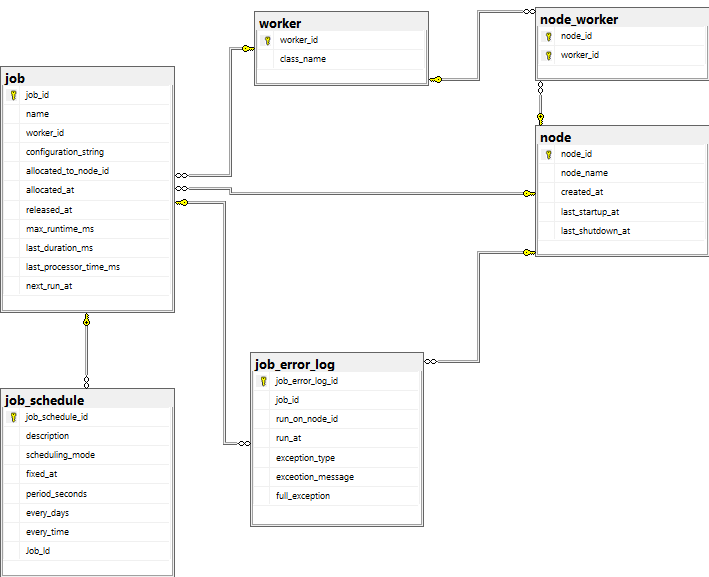
\includegraphics[width=0.7\linewidth]{images/dbmodel.png}
	\caption{Datenbankmodell, eigene Darstellung}
	\label{fig:dbmodel}
\end{figure}
Folgende Entitäten finden sich im Datenmodell:
\begin{itemize}
	\item worker - Enthält den Klassennamen der Instanz die die Abarbeitung der Arbeit der jobs übernehmen.
	\item node - Enthält einen Eintrag für jeden Server der eine Instanz von dJob ausführt.
	\item node\_worker - Ist eine \emph{intersection table}\footnote{Mithilfe einer intersection table wird eine m:n Beziehung zwischen Entitäten dargestellt.\parencite{oracle_intersection}} die die in einer Instanz verfügbaren Worker enthält.
	\item job - Enthält die Jobs die auszuführen sind. 
	\item job\_schedule - Enthält zu jedem Job ein oder mehrere Ausführungszeitpunkte oder einen Hinweis wie der job zu verplanen ist (\code{scheduling\_mode}).
	\item job\_error\_log - Enthält Details zu Fehlern (Exceptions) die während der Ausführung aufgetreten sind. Damit kann der Administrator den Grund für den Fehler feststellen.\footnote{Hier wurde das Protokollieren in die Datenbank gewählt da dies im Gegensatz zu einer Protokolldatei leichter in einer verteilten Umgebung zugänglich ist.}
\end{itemize}
Die Primärschlüssel in den Tabellen wurden als \emph{Unique Identifier} umgesetzt. Dies ist eine Zeichenfolge die errechnet werden kann. Diese hat den Vorteil gegenüber einer numerischen \emph{Identity}, also einem eindeutigen, monoton steigendem Wert der beim Einfügen in die Datenbank durch diese vergeben wird, dass im Falle von verteilten Systemen die Erstellung der Id weniger aufwendig ist, da diese ohne Synchronisierung auf der verteilten Datenbankinstanzen errechnet werden kann. Bei der Verwendung von Identities müssen die Werte, da sie ja eindeutig sein müssen, zwischen den Instanzen synchronisiert werden, was einen Mehraufwand bedeutet. 
\\Der Nachteil der sich unter Umständen aus der Verschlechterung des Index aus der stärkeren Streuung der Werte gibt, wird in diesem Fall in Kauf genommen da in der Regel für den Zugriff andere Indices verwendet werden.\parencite{ms_guid}
\subsection{Zugriff}
Der Zugriff auf die Datenbank erfolgt mittels dem Microsoft Entity Framework (im folgenden kurz EF) in der Version 6. Dies ist eine \emph{ORM (Object Relational Mapping)} Bibliothek die die Datenbank hinter einer Zugriffsschicht verbirgt und die relationalen Daten (Datensätze) direkt in Objekte umwandelt. Damit ist für den Entwickler kein Bruch zwischen Datenbank und objektorientierter Anwendungsentwicklung erkennbar.
\\Dieser Ansatz wird in der Umsetzung vollständig verfolgt in dem die so genannte \emph{code-first} Methode verwendet wird. Dabei
werden die Entitäten als C\# Klassen definiert und automatisch durch das EF die Datenbank erzeugt. 
\begin{lstlisting}[caption={Klassendefinition für Code-First, siehe Job.cs}, label={lst:codefirst}, captionpos=b]
    [Table("job")]
	public class Job
	{
		[Key]
		[Column("job_id")]
		[DatabaseGenerated( DatabaseGeneratedOption.Identity )]
		public Guid Id { get; protected set; }

		[Required]
		[MinLength(8)]
		[MaxLength(64)]
		[Column("name")]
		public string Name { get; protected set; }

		[Required]
		[Column("worker_id")]
		public Guid WorkerRef { get; protected set; }

		[ForeignKey("WorkerRef")]
		public virtual Worker Worker { get; set; }

		[Column("configuration_string")]
		public string ConfigurationString { get; set; }

		[Column("allocated_to_node_id")]
		public Guid? AllocatedToRef { get; protected set; }

		[ForeignKey(nameof( AllocatedToRef ) )]
		public virtual Node AllocatedTo { get; protected set; }

		[Column("allocated_at")]
		public DateTime? AllocatedAt { get; protected set; }

		[Column( "released_at" )]
		public DateTime? ReleasedAt { get; protected set; }
		
		// lines ommited
		
		public virtual ICollection<JobSchedule> Schedule { get; protected set; }
		
		//lines omitted
}
\end{lstlisting}
Über \emph{Annotierungen} können Eigenschaften in der Umsetzung geändert werden (siehe \parencite{eftut}). Mit den Annotierungen \code{Table} und \code{Column} können die Namen der Tabellen und Felder geändert werden. Für die Eigenschaft \code{Id}  werden zusätzlich die Annotierungen \code{Key} um diese als Primärschlüssel zu kennzeichnen, und \code{DatabaseGenerated} verwendet. Damit wird - da es sich um einen Unique Identifier handelt - ein default-Wert für die Spalte von \code{newsequentialid()} erzeugt. Die Datenbank generiert somit den Primärschlüssel selbst. \code{Required} definiert für die Eigenschaft \code{Name} eine not-null Beschränkung, der Wert muss also im Datensatz vorhanden sein. Zusätzlich sind für diese Eigenschaften noch eine minimale und maximale Länge gesetzt. Dies ist bei String-Typen von Bedeutung, da sonst automatisch ein String mit maximaler Länge in der Datenbank angelegt wird, was negative Auswirkungen auf die Laufzeit haben kann. 
\\Von Bedeutung sind auch die \code{virtual} Modifikatoren. Diese weisen das EF an, die Inhalte der Eigenschaften erst beim tatsächlichen Zugriff auf diese zu laden. Dies wird als \emph{lazy loading} bezeichnet. Damit werden Daten aus verbundenen Tabellen nur dann geladen, wenn diese benötigt wird. Ohne das lazy loading würden die Daten immer geladen werden, auch wenn diese gar nicht benötigt werden. Durch die Nutzung dieser Methode kann das verhalten zur Laufzeit verbessert werden da keine unnötigen Daten in der Datenbank gelesen werden. Die technische Umsetzung in EF erfolgt mittels des so genannten \emph{Proxy-Patterns} \footnote{ siehe \parencite[S. 207ff]{gamma1995}}\parencite{ms_proxy}. Dabei wird dynamisch durch das EF eine Instanz einer Klasse erzeugt die von der Entität erbt. Um das lazy loading zu Implementieren, werden in den Zugriffsfunktionen der Proxy-Klasse zuerst die Daten von der Datenbank geladen und erst danach an den Aufrufer zurückgegeben.
\\Der Zugriff auf die Daten erfolgt über einen so genannten \code{Context} der die notwendigen Operationen durchführt und die geladenen Objekte gegebenenfalls anreichert. Der Context speichert auch alle geladenen Objekte und erkennt und verfolgt Änderungen an den Objekten so dass alle Änderungen an geladenen Objekten über den Context mit einem einzigen Befehl (\code{Context.SaveChanges()}) gespeichert werden können.
\\Geladen werden die Abfragen über die C\# Spracherweiterung \emph{LINQ}\footnote{Language INtegrated Query - siehe \url{https://docs.microsoft.com/en-us/dotnet/csharp/programming-guide/concepts/linq/}}. Diese datenbankunabhängige Abfragesprache wird durch das EF in SQL übersetzt. Daher wird LINQ auch für Abfragen in interne Collections wie Listen verwendet.
\begin{lstlisting}[caption={LINQ Abfrage - Lambda Syntax, siehe DefaultJobLoader.cs - DoLoad()},label={lst:linq_fluent},captionpos=b]
	var q = dbContext.Jobs.Include( "Worker" )
			.Where( j => myNextJobIds.Contains( j.Id ) )
			.OrderBy( j => j.NextRunAt )
			.AsNoTracking( )
			;

\end{lstlisting}
Wie in Listings \ref{lst:linq_fluent} und \ref{lst:linq_expression} dargestellt ist, verfügt LINQ über zwei unterschiedliche Formen. Die so genannte \emph{Lambda} Syntax, bei der die Syntax der C\# Sprache beibehalten wird und \emph{Lambdas} einsetzt um Operationen durchzuführen. Und die \emph{Query Expression} Syntax, bei der eine SQL ähnliche Abfrage direkt im Code geschrieben werden kann. Beide Varianten sind in etwa gleich mächtig\footnote{Einige Funktionen stehen nur in der Lambda Syntax zur Verfügung} und können auch abwechselnd verwendet werden.\footnote{Die Query Expression Syntax ist genau genommen nur eine Syntax Erweiterung und wird in eine Lambda Expression umgewandelt.\parencite{linq}}
\begin{lstlisting}[caption={LINQ Abfrage - Query Expression Syntax},label={lst:linq_expression},captionpos=b]
	var q = from job in dbContext.Jobs
			where myNextJobIds.Contains( job.Id ) )
			orderby job.NextRunAt
			select job
		;
\end{lstlisting}
Zeile 1 in Listing \ref{lst:linq_fluent} definiert die Tabelle aus der die Daten geladen werden sollen. Die Erweiterung \code{.Include("Worker")} weist das EF an, die Daten der Eigenschaft \code{Worker} aus der verbundenen Tabelle ebenso gleich zu laden. Dies nennt man \emph{eager loading}. Damit werden alle Daten in einer Abfrage geladen, was positive Auswirkungen auf die Laufzeit hat.\footnote{Die Eigenschaft \code{Worker} ist virtuell und wird daher erst beim Zugriff geladen. Da aber an dieser Stelle im Code die Daten der \code{Worker} Eigenschaft benötigt werden, wird hier ein eager-loading erzwungen um performanter zu sein.}
\subsubsection{Laden der Jobs}
Das Laden der Jobs die ausgeführt werden sollen ist eine der kritischsten Stellen. Die Jobs müssen so rasch wie möglich geladen werden, ohne aber dabei andere laufende Instanzen zu behindern. Dies wird Mithilfe der Nutzung von Isolation Levels und Sperren erreicht. Dies ist nur mithilfe eines SQL Statements möglich, EF bietet auf dieser Ebene keine Unterstützung an.
\begin{lstlisting}[caption={Jobs Laden, siehe DefaultJobLoader.cs - DoLoad()},label={lst:jobloader},captionpos=b]
string loadCommand = $@"SELECT TOP {gulpSize}
				job.job_id
				, job.name
				, node.node_name
				FROM job
				WITH (XLOCK, ROWLOCK, READCOMMITTED , READPAST)
					JOIN node_worker ON ( node_worker.worker_id = job.worker_id )
					JOIN node ON ( node.node_id = node_worker.node_id AND node.node_name = @NodeId)
				WHERE job.allocated_to_node_id IS NULL
					AND job.next_run_at < CURRENT_TIMESTAMP
				ORDER BY job.next_run_at ASC";
\end{lstlisting}
Mit dem Statement in Codebeispiel \ref{lst:jobloader} werden die Id's der nächsten Jobs gelesen die auszuführen sind. Mit dem \code{join} der node\_worker Tabelle werden dabei nur die jobs berücksichtigt, die in dieser Instanz ausgeführt werden können. Die Abfrage \code{allocated\_to IS NULL} schließt Jobs aus die bereits in anderen Instanzen geladen sind. 
\\Die sogenannten \emph{Hinweise (hints)} (siehe \parencite{ms_hints}) in Zeile 6 wird das verhalten bei Nebenläufigkeit gesteuert.
\begin{itemize}
	\item \code{READCOMMITED} - Setzt die Isolationsstufe für dieses Statement. Damit werden Änderungen von anderen committeten Transaktionen gelesen, auch wenn diese nach dem Start der eigenen Transaktion erst committed wurden.\footnote{Siehe Kapitel \ref{subs:isolation}.} Die Isolationsstufe wird hier erzwungen, damit READPAST immer fehlerfrei angewendet werden kann.
	\item \code{READPAST} - Damit werden von anderen Transaktionen gesperrte Datensätze ignoriert und die Datensätze nach dem gesperrten gelesen. Ansonsten würde die Transaktion warten bis die Sperre auf dem Datensatz aufgehoben ist.
	\item \code{ROWLOCK} - Setzt eine Sperre auf Datensatzebene auf die gelesenen Datensätze.
	\item \code{XLOCK} - Weist die Datenbank an ein Exklusive Sperre zu setzen. Damit kann der Datensatz von keiner anderen Transaktion gelesen werden.
\end{itemize}
Nachdem die Jobs geladen wurden, werden sie in der selben Transaktion durch das setzen des Feldes \code{allocated\_to} logisch gesperrt und von anderen Instanzen nicht mehr geladen. Diese Vorgehensweise stellt sicher dass die Jobs nur von einer Instanz gelesen werden, aber andere Instanzen weitere auszuführende Jobs lesen kann. Die Anzahl der Jobs die gelesen werden ist durch die \code{TOP} Klausel beschränkt die von Administrator konfiguriert werden kann.\footnote{Diese Art der Übergabe von Parametern ist prinzipiell ein Sicherheitsrisiko (\emph{SQL-Injection}). Da der Parameter ein Integer Wert ist und dies durch die Anwendung sichergestellt ist, ist das Statement trotzdem sicher.}
\\Um die Transaktion so klein wie möglich zu halten und somit die gesetzten Datenbanksperren so kurz wie möglich zu halten, endet die Transaktion nach dem setzen der Node. In einer zweiten Transaktion danach werden erst die vollständigen Daten der allokierten Jobs geladen.
\\Nachdem alle Jobs geladen wurden, werden diese dem Arbeitsvorrat hinzugefügt. Die Details dazu sind in den Kapiteln \ref{sec:producerconsumer} und \ref{sec:blockingq} beschrieben.
\section{Skalierung}
Einer der ausschlaggebenden Gründe für die Entwicklung war, dass bisherige Lösungen hinsichtlich der Leistung schlecht skalieren. Die einzige Möglichkeit ist meist, einen stärkeren Server zu nutzen. Deswegen ist die leichte Skalierung der Leistung eine grundlegende Anforderung an das System. Um bestimmte Aufgaben effizient abarbeiten zu können, kann es notwendig sein, eine darauf ausgelegt Hardware zu verwenden, um in etwa Berechnungen auf einer GPU durchzuführen. Dies wird mit der Möglichkeit der funktionalen Skalierung erreicht.
\subsection{Skalierung der Leistung} \label{sec:scaling}
Das umgesetzte System bietet zwei Möglichkeiten die Leistung zu skalieren. Die erste Möglichkeit ist die Skalierung der Leistung innerhalb eines Servers durch die Konfiguration der maximal gleichzeitig laufenden Threads pro Instanz. Damit kann die für dJob zur Verfügung stehende Leistung sowohl erhöht, als auch beschränkt werden um andere, am selben Server laufende Applikationen nicht zu beeinflussen.
\\Die zweite Möglichkeit ist die Nutzung von mehren Servern. Dies ist durch dJob durch Installation des Services und der benötigten Worker erledigt. Es sind keinerlei weitere Anpassungen oder Konfigurationen nötig um das System zum Laufen zu bringen. 
\\Für die Installation gibt es drei grundlegende Möglichkeiten (siehe auch Darstellung \ref{fig:performance_scaling}):
\begin{enumerate}
	\item Szenario 1 - Ein Server, Datenbank und Applikation ist am selben Server installiert. Damit können kleine Systeme mit geringen Leistungsanforderungen umgesetzt werden.
	\item Szenario 2 - Mehrere Server, auf einem Server ist die Datenbank und die Applikation installiert, auf den restlichen Servern ist nur die Applikation installiert. Damit können mittlere Systeme, oder Systeme mit spezialisierter Hardware umgesetzt werden.
	\item Szenario 3 - Mehrere Server auf denen die Applikation installiert ist und die auf eine verteilte Datenbank auf mehreren Servern zugreifen. Damit können größte und weltweit verteilte Systeme umgesetzt werden.
\end{enumerate}
Durch die Verwendung eines Datenbanksystems zur Speicherung der Jobs ist die Konfiguration des dJob Services in allen Szenarien gleich. Es muss lediglich der \emph{connection string} der die Verbindung zur Datenbank definiert korrekt konfiguriert werden. Für das System und für die einzelnen Instanz hat das gewählte Szenario kein Auswirkungen und ist für die Anwendung auch nicht merkbar. Die Probleme die durch die Gleichzeitigkeit entstehen sind in der Datenbank und durch die Umsetzung des Ladens der Jobs abgefangen. 
\\Im dritten Szenario liegt die Komplexität der Konfiguration außerhalb des Systems bei der verteilten Datenbank. Dies kann in SQL-Server mittels einer \emph{transactional replication} zwischen Servern.\parencite{ms_resolve} Damit werden alle Daten in den Datenbanken und alle Daten die zur Verwaltung nötig sind (wie in etwa Sperren) zwischen den einzelnen Servern automatisch aktualisiert. Aus Sicht der Applikation ändert sich nichts, da eine verteilte Datenbank sich gegenüber Anwendungen wie eine einzelne Instanz verhält. Eine Variante des dritten Szenarios ist die Verwendung einer Cloud-basierten Datenbank. Diese ist aus Sicht der Applikation ident mit Szenario 3. Um bei der Verwendung einer Cloud-Datenbank immer genügend Arbeitsvorrat in einer Instanz zur Verfügung zu haben, kann es notwendig sein eine höhere \code{gulpSize} und eine höhere \code{lowWaterMark}\footnote{Das ist die Anzahl an Jobs im Arbeitsvorrat die unterschritten sein muss bevor neue Jobs geladen werden.} zu konfigurieren. Damit kann eine längere Dauer des Ladens der Jobs abgefangen werden.
\\In der beispielhaften Verwendung wurde das Szenario 2 umgesetzt und erreicht die derzeit nötige Leistung mit 3 Servern mit je 8 Kernen die über Österreich verteilt genutzt werden.
\begin{figure}
	\centering
	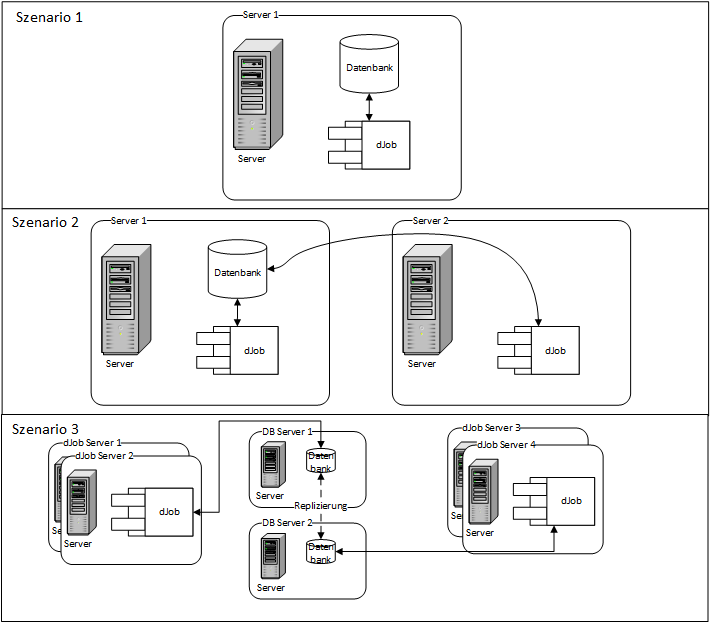
\includegraphics[width=0.7\linewidth]{images/scaling}
	\caption{Skalierung der Leistung, eigene Darstellung}
	\label{fig:performance_scaling}
\end{figure}

\subsection{Funktionale Skalierung} \label{sec:dynload}
Mithilfe der funktionalen Skalierungen werden zwei grundlegende Anforderungen erfüllt. Es können weitere Worker, also die Funktionen die die tatsächliche Arbeit verrichten, ohne Veränderung des dJob Systems umgesetzt werden, und die einzelnen dJob Instanzen können über unterschiedliche Worker besitzen um differenzierte Hardware der Server auszunutzen.
\\Um neue Worker zu definieren, müssen diese in einer \emph{\.NET Assembly} vorhanden sein. 
Diese ist die kleinste Einheit in der Code zur Verfügung gestellt werden kann. Sie enthält neben dem Programmcode\footnote{Dieser ist in der Assembly bereits in die \emph{Intermediate Language (IL)} kompiliert.} auch Metadaten, die unter anderem auch die Abhängigkeiten zu anderen Assemblies definieren. Eine Assembly wird typischerweise als eine Bibliothek (.dll) oder als direkt ausführbares Programm zur Verfügung (.exe) gestellt \parencite[S. 17ff]{box}. Das dJob Service wird als ausführbares Programm zur Verfügung gestellt, alle Assemblies von denen es abhängig ist, sind entweder .NET Standard-Assemblies oder, wie die dJob.core Bibliothek im selben Verzeichnis vorhanden und können somit durch .NET selbst geladen werden. Die Abhängigkeiten zu diesen Assemblies wird zum Zeitpunkt der Kompilierung ermittelt und in den Metadaten der .exe Datei gespeichert.
\\Um Programmcode zu nutzen der zum Zeitpunkt der Kompilierung nicht Teil von dJob war, müssen diese Assemblies zur Laufzeit \emph{dynamisch} geladen werden.Das dJob service sucht dazu in einem konfiguriertem Pfad alle Programmbibliotheken und lädt diese Assemblies in den Speicher, dies ist in Codebeispiel \ref{lst:dynamicloading} dargestellt. 
Worker - Klassen in den Bibliotheken die die Arbeit erledigen, müssen dabei \begin{enumerate}
	\item von außerhalb der Bibliothek sichtbar sein - nur so kann eine Klasse instanziiert werden
	\item vom Interface \code{at.loe.djob.core.worker.IWorker} erben
	\item einen parameterlosen Konstruktor haben.
\end{enumerate}
Alle im Verzeichnis vorhandenen Bibliotheken (Zeile 1) werden geladen (Zeile 3). Danach werden alle Klassen die das Interface \code{IWorker} implementieren (Zeile 5\&6) instantiiert (Zeile 8) und in einer Collection\footnote{Es handelt sich um ein \code{ConcurrentDictionary}. Dies ist eine Key/ Value Sammlung mit eindeutigen Keys die für die Verwendung durch mehrere Threads vorgesehen ist. Die Zugriffe auf die Collection sind immer thread-safe, alle eventuell notwendigen Sperren werden durch die Collection selbst verwaltet.} abgelegt (Zeile 12).
\begin{lstlisting}[caption={Dynamic Loading, siehe WorkerRepository.cs - LoadAllWorkers()},label={lst:dynamicloading},captionpos=b]
foreach ( string file in  workerDirectory.GetFiles( "*.dll" ) )
{
	Assembly assembly = Assembly.LoadFile( file );

	foreach ( Type typeToLoad in assembly.GetTypes()
					.Where( t => t.ImplementsInterface<IWorker>() ) )
	{
		IWorker w = (IWorker)Activator.CreateInstance( typeToLoad );

		w.Initialize( ObjectRepository.Get<IConfigurationProvider>( ), logger );

		if( ! repository.TryAdd( typeToLoad.FullName, w ) )
		{
			throw new InvalidOperationException
			( $"Could not add class '{typeToLoad.FullName}' to repository");
		}
	}
}
\end{lstlisting}
Wenn die Bibliotheken die geladen werden sollen Abhängigkeiten zu anderen, nicht-Standard, Bibliotheken haben, so werden diese nur automatisiert aufgelöst und geladen wenn diese entweder global verfügbar sind oder in Verzeichnis des Services zu finden sind \parencite[S. 42ff]{box}). Liegen diese im Verzeichnis in dem auch die Worker-Bibliothek abgelegt ist, so muss diese Auflösung durch die Anwendung selbst erfolgen. Dafür stellt .NET das Ereignis \code{AssemblyResolve} zur Verfügung. Die Anwendung kann dann die benötigten Bibliotheken selbst suchen und laden\footnote{Siehe WorkerRepository.cs Methode \code{LoadDependentAssembly()}} \footnote{Wird dies nicht durch die Anwendung erledigt, so erhält man eine \code{FileNotFoundException} mit dem Name der Bibliothek \emph{die den Verweis enthält}, und nicht, den Namen der Bibliothek die nicht aufgelöst werden kann. }.
\\Nachdem alle Worker geladen wurde, werden diese in der Datenbank für die aktuelle Instanz aktualisiert, so dass beim Laden der Jobs für die Instanz nur diese Jobs geladen werden die auch ausgeführt werden können. Dadurch können für jede Instanz unterschiedliche Worker konfiguriert werden, was die zweite Anforderung abdeckt.
\section{Concurrency}
Um die Leistung eines Servers ausnutzen zu können werden die geladenen Jobs durch mehrere Threads parallel abgearbeitet. Dazu werden durch den \code{DefaultJobScheduler} die konfigurierte Anzahl an Threads angelegt und gestartet. Diese beziehen ihre Arbeit aus einer globalen Datenstruktur die Jobs und führen dann die für die Jobs konfigurierten Worker aus. Diese Architektur entspricht dem \emph{Producer/ Consumer Pattern} \parencite[S. 163ff]{jthreads}. Der \code{DefaultJobLoader} entspricht dabei dem Producer, die einzelnen \code{JobWorker} dabei den Consumern. Ein entscheidendes Element dieses Patterns ist die Datenstruktur die für die Entkopplung sorgt. Durch den Zugriff mehrere Threads muss diese einerseits thread-safe sein, andererseits müssen die Operationen so effizient wie möglich sein. Daher werden diese zwei Element näher betrachtet.
\subsection{Producer-Consumer}\label{sec:producerconsumer}
Der Producer/ Consumer Pattern ist einer der häufigst verwendeten Pattern wenn es um Abarbeitung von Aufgaben durch mehrere Threads geht. Er besteht aus 
\begin{itemize}
	\item ein oder mehreren Producern die in eigenen Threads laufen und Arbeitspakete produzieren
	\item einer zentralen Datenstruktur, in die Producer die Arbeitspakete einfügen und die Consumer diese entfernen
	\item ein oder mehrere Consumer, die wiederum als eigene Threads laufen und die Arbeitspakete aus der zentralen Datenstruktur holen und abarbeiten.
\end{itemize}
Dies ist auch in Abbildung \ref{fig:architecture} dargestellt.\parencite{jthreads}
\begin{figure}
	\centering
	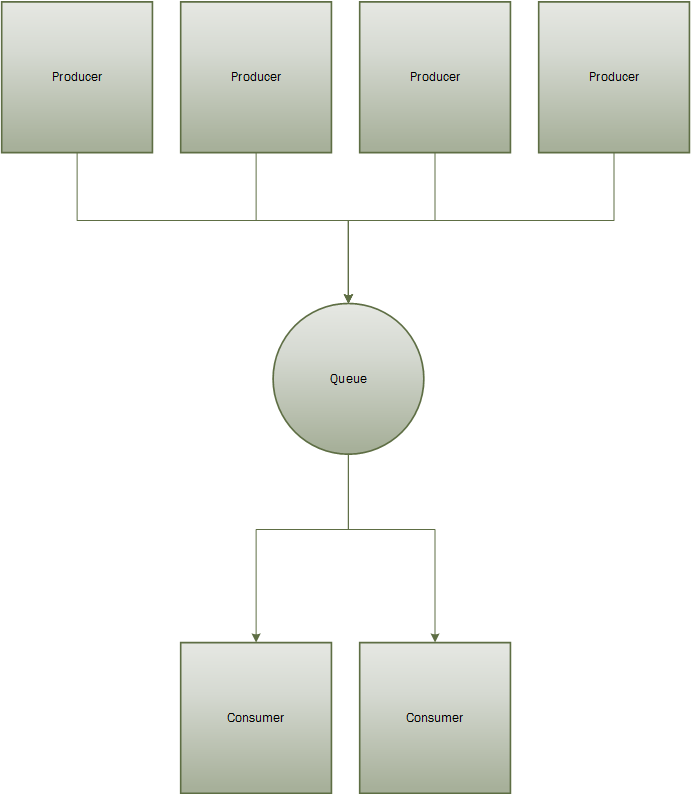
\includegraphics[width=0.7\linewidth]{images/B2_Producer_Consumer_1}
	\caption{Producer/ Consumer Darstellung, vgl. \parencite[S. 163]{jthreads}}
	\label{fig:architecture}
\end{figure}
\\Die Verbreitung dürfte in seiner Einfachheit begründet sein. Denn sowohl Producer als auch Consumer, die jeweils in verschiedenen Threads ihre Arbeit verrichten brauchen beim Zugriff auf die Daten keine weiteren Aktionen durchführen\footnote{Dies gilt für die zu bearbeitenden Daten, beim Zugriff auf andere, globale Daten sind diese sehr wohl Sperren zu setzen.} \parencite[S. 163ff]{jthreads}. Der Schutz der Daten des Arbeitspaketes erfolgt durch die Datenstruktur, in der Regel eine Queue. Diese setzt innerhalb der öffentlichen Methoden die Sperren wenn nötig. Diese übernimmt auch die Aufgabe des Aufweckens von Consumern wenn Arbeit anliegt.
\\Der Pattern ist auch sehr vielseitig. In einer weiteren gebräuchlichen Form (siehe Abbildung \ref{fig:architecture_2}) ist die Verwendung von mehreren Queues und einem Dispatcher. Dies kann einerseits bei einer sehr hohen Anzahl an Producern oder Consumern verwendet werden, da dadurch die Häufigkeit der Sperren, und damit die Wartezeit eines Threads gesenkt wird. Weiters kann auch die Anzahl an Consumern pro Queue unterschiedlich sein. Damit kann der Dispatcher wichtigere Arbeitsaufgaben in die Queue legen der mehr Consumer zugeteilt sind. Damit erfolgt eine schnellere Abarbeitung des Arbeitspaketes.
\begin{figure}
	\centering
	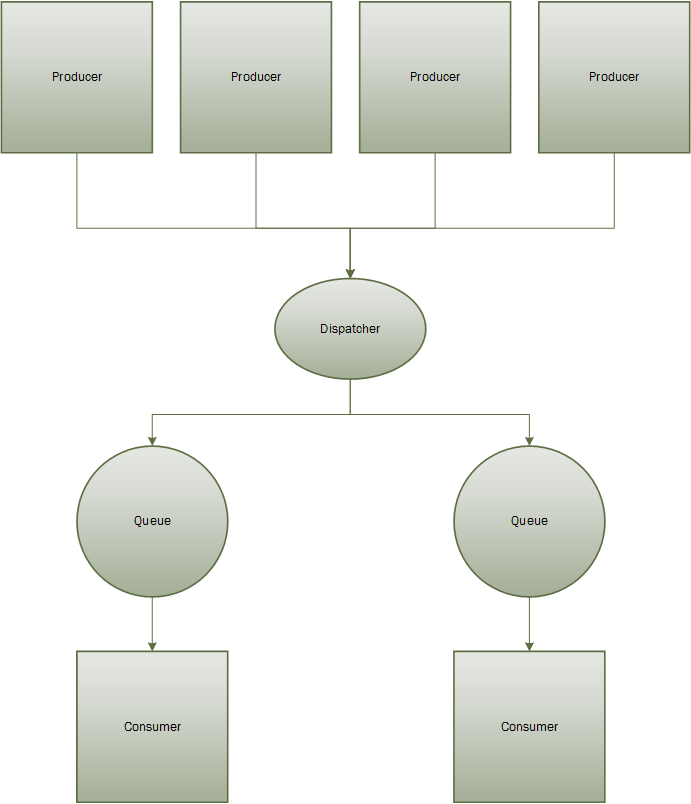
\includegraphics[width=0.7\linewidth]{images/pc_w_dispatcher}
	\caption{Producer/ Consumer Darstellung mit mehreren Queues, vgl. \parencite[S. 163]{jthreads}}
	\label{fig:architecture_2}
\end{figure}
\\Im dJob Service ist die Implementation des \code{IJobLoader} der einzelne Producer. Die vorab allokierten und gestarteten Instanzen der \code{JobWorker} bilden die Producer. Die zentrale Datenstruktur ist die \code{BlockingCollection} namens \code{pendingWork}.
\subsection{BlockingCollection}\label{sec:blockingq}
Wie im vorigen Kapitel beschrieben, leistet die zentrale Datenstruktur im Producer/ Consumer Pattern den Großteil der Arbeit was die Synchronisierung der einzelnen Threads betrifft. Daher ist das Design und die Implementierung dieser Klasse essentiell für die Leistung des Gesamtsystems. Die Klasse muss
\begin{itemize}
	\item sicherstellen dass die Methode zum Einfügen der Elemente thread-safe ist, also mehrere Threads zugleich Elemente einfügen können ohne die Datenstruktur zu beschädigen
	\item sicherstellen, dass die Methode zum Entfernen der Elemente thread-safe ist
	\item Consumer Threads suspendieren wenn keine weitere Arbeit anliegt
	\item Consumer Threads aufwecken wenn weitere Arbeit eingefügt wurde
	\item die Anzahl an gesetzten Sperren und die Zeitdauer der Sperre so gering wie möglich halten.
\end{itemize}
Codebeispiel \ref{lst:blockingQ} zeigt die Implementierung einer solchen Klasse. Zur Datenhaltung wird die Standardklasse \code{Queue} verwendet (\code{backingStore}), die selbst nicht thread-safe ist.
\begin{lstlisting}[caption={Implementierung BlockingQ, siehe MyBlockingQ.cs}, label={lst:blockingQ}, captionpos=b]
    public class MyBlockingQueue<T>
	{
		private Queue<T> backingStore = new Queue<T>();

		/// <summary>
		/// lock to protect the backingStore and used for notifications
		/// </summary>
		private readonly object myLock = new object();

		public MyBlockingQueue()
		{ /* empty */ }


		/// <summary>
		/// add an item to the queue in a threadsafe way
		/// </summary>
		public void Enque( T newElement )
		{
			lock( myLock )
			{
				backingStore.Enqueue( newElement );

				Monitor.Pulse( myLock );
			}
		}

		/// <summary>
		/// Take an item from the queue
		/// if no item is available, wait until an element has been put into the queue and check again
		/// </summary>
		/// <returns>an element from the q</returns>
		public T Dequeue( int millisecondsTimeout )
		{
			lock( myLock )
			{

				while ( ! backingStore.Any() )
				{
					if( !Monitor.Wait( myLock, millisecondsTimeout ) )
					{
						return default( T );
					}
				}

				return backingStore.Dequeue();
			}
		}
}
\end{lstlisting}
Die gezeigte Implementierung erfüllt alle genannten Bedingungen. In der Methode \code{Enque} wird innerhalb einer gesetzten Sperre ein Element der Sammlung hinzugefügt(Zeile 21). Und danach mittels eines Monitors ein suspendierter Consumer geweckt (Zeile 23)\footnote{Sollte kein Consumer suspendiert sein, so erfolgt keine Aktion.}. 
Die Consumer rufen die Methode \code{Deque} auf und erhalten entweder eine Element oder werden suspendiert. In der Methode wird eine Sperre gesetzt (Zeile 34) und danach geprüft ob Elemente vorhanden sind (Zeile 37). Wenn Elemente vorhanden sind, wird das erste Element der Queue zurückgegeben (Zeile 42). Wenn kein Element vorhanden ist, so wird auf das Einfügen eines Elementes gewartet (Zeile 39). Wird der Thread aufgeweckt, so wird nochmals geprüft ob Elemente vorhanden sind und erst danach das erste Element zurückgegeben\footnote{Ein anderer Consumer könnte das Element welches das Aufwecken ausgelöst hat bereits abgearbeitet haben, siehe dazu auch \ref{sss:Monitore}}. Um steuern zu können wie lange die einzelnen Consumer warten, kann eine Zeit in Millisekunden angegeben werden die gewartet wird. Wird innerhalb der Zeitspanne kein neues Element eingefügt, so wird der Default-Wert des Typs zurückgegeben.
\\Diese Umsetzung ist an sich korrekt, ist jedoch für die Verwendung in Produktivsystemen nur bedingt geeignet, da zum Erreichen der thread-Sicherheit immer Sperren verwendet werden. Diese Sperren bedingen aber auch immer einen zusätzlichen Aufwand der innerhalb des Betriebssystems entsteht. Aus diesem Grund wurde in der Umsetzung nicht die dargestellte Umsetzung gewählt, sondern die \code{BlockingCollection} aus der .NET Standardbibliothek\footnote{Siehe \parencite{ms_blockingcollection}}. Diese verwendet als Datenspeicher eine Instanz der Klasse \code{BlockingQueue} \footnote{Siehe \parencite{ms_concurrentq}} 
\\Diese Implementierung hat entscheidende Vorteile:
\begin{itemize}
	\item Es wird nicht eine Datenstruktur zur Speicherung genutzt, sondern die Daten auf mehrere Segmente aufgeteilt. Damit erfolgt eine Entkopplung zwischen dem Einfügen und dem Entfernen aus der Sammlung. Dies bringt den Vorteil, dass die einzelnen Datenstrukturen von weniger Threads benötigt werden, wodurch die Anzahl der Möglichen Konflikte und damit auch die Notwendigkeit mit race-conditions umzugehen reduziert. Dies ist in der Klasse \code{BlockingCollection} in den Methode \code{TryAdd} und \code{TryTake} zu sehen. Wenn mehr als \code{SEGMENT\_SIZE} Elemente eingefügt wurden, wird ein neues \code{Segment} verwendet.
	\item Die Implementierung ist \emph{lock\-free}. Sie ist gänzlich ohne Sperren umgesetzt, was den Vorteil hat, dass der Zusatzaufwand zum Setzen und Entfernen der Sperren vermieden wird. Dazu werden atomare Operationen genutzt\footnote{Die Methoden sind in der Klasse \code{Interlocked} implementiert.} um lokale Sperrvariablen zu setzen. Wenn diese Sperren gesetzt sind, und daher zu diesem Zeitpunkt kein Zugriff auf die Daten erfolgen darf, werden \emph{SpinLocks} verwendet um zu warten bis die Datenstrukturen wieder entsperrt sind. SpinLocks sind optimierte Sperren, bei denen zuerst eine Schleife durchlaufen wird um zu warten\footnote{Dieses so genannte busy-wait ist - auf wenige Iterationen beschränkt - in einer Multipozessor-Umgebung ressourcensparender als das Setzen einer Sperre \parencite[S. 70]{masterk}.} 
\end{itemize}


\subsection{Verwendung der .NET Bibliothek für parallele Aufgaben}
.Net bietet zur asynchronen Abarbeitung von Aufgaben seit der Version 4 eine eigene Bibliothek, die \emph{Task Parallel Library (TPL)}\footnote{Siehe \url{https://msdn.microsoft.com/de-de/library/dd460717(v=vs.110).aspx}}. Diese und die Schlüsselwörtar \code{async/ await} ermöglichen es, Aufgaben sehr einfach parallel abzuarbeiten. Damit könnte der Scheduler wie in Codebeispiel \ref{lst:tpl} dargestellt umgesetzt werden. In Zeile 9 werden dabei die geladenen Jobs durch mehrere Threads parallel \code{Parallel.ForEach} ausgeführt.
\\Da hier sehr viele Elemente versteckt in einer Standard-Bibliothek ablaufen und über weite Strecken die Transparenz und die Tuning-Möglichkeiten durch die Anwendung nicht mehr gegeben sind, wurde eine Umsetzung mittels TPL bewusst nicht gewählt.

\begin{lstlisting}[caption={JobScheduler, einfache TPL Implementierung, siehe SimpleTpl.cs}, label={lst:tpl}, captionpos=b]
public class SimpleTpl<T>
{
	private volatile bool isRunning = true;
	
	public void Start()
	{
		while ( isRunning )
		{
			Parallel.ForEach( LoadWork(), j => ProcessJob( j ) );
		}
	}
	
	private void ProcessJob( T job )
	{
		//execute job
	}
	
	private List<T> LoadWork()
	{
		//load from db or sleep and try again
		return new List<T>();
	}
	
	public void Stop() => isRunning = false;
}
\end{lstlisting}
\chapterend
  
  \selectlanguage{german}
%-----------------------------------------------------------------------------
\chapter{Konklusio}\label{chap:Konklusio}
%-----------------------------------------------------------------------------
\chapterstart

\section{Zusammenfassung}
Im Rahmen dieser Arbeit wurden einige theoretischen Grundlagen für wichtige Techniken zur Umsetzung von performanten Anwendungen gezeigt. Dies waren vor allem der Umgang mit mehreren Threads und die Grundlagen von parallelem Zugriff auf Datenbanksysteme. Diese Techniken wurden verwendet um ein System zur verteilten Ausführung von Aufgaben umzusetzen. Durch die Nutzung eines Datenbanksystemes konnten die Aufgabenstellungen zur Datenspeicherung und zur Verteilung der Aufgaben über mehrere Server gelöst werden. Das entwickelte Service nutzt die Technik des dynamischen Ladens von Programmteilen um neue Arten von Aufgaben ohne Änderung des Programmcodes des Services zu ermöglichen. Das Abarbeiten der Aufgaben wurde mit einem Procuder/ Consumer Pattern um gesetzt, um so die Leistung des jeweiligen Servers optimal ausnutzen zu können.
\\Die Anwendung der jeweiligen Techniken und Vor- oder Nachteile wurden in der Umsetzung beschrieben um für den Leser die Umsetzung verständlich zu machen.
\\Das entwickelte Service sowie außerhalb dieser Arbeit entwickelte Worker zur Skalierung von Bildern werden in einer beispielhaften Umsetzung verwendet um die Brauchbarkeit des Systems in der Praxis zu testen. Dabei werden auf drei Servern auf Österreich verteilt Daten von mehr als 1.000 Messstationen verarbeitet. Es dabei in fixen Zeitabständen unter anderem Bilddaten von den einzelnen Stationen geholt und danach in verschiedene Auflösungen umgerechnet und abgelegt. Im Rahmen des Hochfahrens des Systems wurde die Anzahl der Server von 2 auf 3 erhöht, da der Aufwand zur Umrechnung der Bilder viel Leistung in Anspruch nahm. Dies war durch die Auslegung des Systems leicht zu bewerkstelligen.
\\Die Eingangs gesetzten Ziele der Arbeit konnten somit erreicht werden.
\chapterend

  \listoffigures
  \lstlistoflistings
  \printbibliography
  
% Add bibliography to table of contents as "References", at chapter level
% Keep this _after_ bibliography, only then the link in the TOC is correct!
\addcontentsline{toc}{chapter}{References}

\end{document}

\selectlanguage{german}

%**********************************************************************
%**********************************************************************